\documentclass[]{article}

\usepackage[title]{appendix}
\usepackage{acronym}
\usepackage{multicol}
\usepackage{graphicx}
\usepackage{rotating}

\usepackage{longtable}
\usepackage{multirow}



\usepackage{chngcntr}


\usepackage[table]{xcolor}

\usepackage[margin=1.25in]{geometry}


%opening
\title{Alberta E-Vent Control Software}
\author{Initial Release and Development Overview for Software Version 042920}

\begin{document}
	


\maketitle

\newpage

\section*{Document History}
\begin{center}
	\begin{tabular}{ |p{3cm}| p{3cm}| p{3cm}| p{3cm}|}
		\hline
		Date & Document Status & Originator & Approver \\
		\hline 
		 \date{\today} & Draft & C. Hill \& D. Quinn &  \\  
		\hline
		 &   &  & \\ 
		 \hline
	\end{tabular}
\end{center}

\section*{Approval}

\begin{center}
	\begin{tabular}{ |p{3cm}| p{3cm}| p{3cm}| p{3cm}|}
		\hline
		Date & Name & Role & Signature \\
		\hline 
		& &  &  \\  [2ex]
		\hline
		&   &  & \\ [2ex]
		\hline 
		&   &  & \\ [2ex]
		\hline   
		&   &  & \\ [2ex]
		\hline     
	\end{tabular}
\end{center}


\clearpage

\tableofcontents

\clearpage


\section{Summary}

This report outlines the Alberta E-Vent software design, development and testing that has been undertaken.  The report is composed of four main parts:
\begin{itemize}
	\item Sections \ref{sect:software_class} to \ref{sect:quality_manage} cover how the development of the software has been undertaken in accordance with the IEC 62304.2006 standard.
	\item Sections \ref{sect:function_overview} to \ref{sect:risk} describes the function and design of the software in detail.
	\item Section \ref{sect:vandv} covers verification and validation testing performed to check the performance of the software.
	\item Section \ref{sect:maintenance} covers the proposed maintenance plan for continuing support of the Alberta E-Vent software.
\end{itemize}

\clearpage

\section{Acronyms}

%\begin{multicols}{2}
\begin{acronym}
	
	\acro{AC}{Assist Control}
	
	\acro{BPM}{Breaths per Minute}
	
	\acro{IT}{Inspiratory Time}
	
	\acro{PEEP}{Positve End-Expiratory Pressure}
	\acro{PIP}{Peak Inspiratory Pressure}
	
	\acro{RR}{Respiratory Rate}
	
	\acro{TP}{Trigger Pressure}
	\acro{TV}{Tidal Volume}
	
	\acro{VC}{Volume Control}
	
\end{acronym}
%\end{multicols}


\clearpage

\section{Software Classification}
\label{sect:software_class}
The Alberta E-Vent has been designed as a emergency ventilation system which requires human supervision. The intent of the system is to offload the physical burden of manually running a bag-valve-mask setup while still utilizing the trained supervision of medical professional. Further, it is expected that the device will be used on patients capable of spontaneous breathing which requires the Assist Control Mode of ventilation.

The Alberta E-Vent utilizes an external mechanical relief valve to limit the maximum operating pressure of the ventilator.  This valve prevents the ventilator from generating pressures that would cause severe harm to the patient.  Further, the ventilator acts as an aid to patient's breathing but does not prevent them from spontaneous inhalation or exhalation during operation.  The anticipated operating conditions of the ventilator, as detailed in the preceding paragraph, would mean that a software malfunction will not cause suffocation.  The primary risks associated with a software failure relate to asynchronous breathing and the associated lung injury associated with this operating condition.  This rationalization provides the justification for treating the software as Class B in accordance with IEC 62304.2006.

\clearpage


\section{IEC 62304.2006 Overview}

The Alberta E-Vent Software has designated Class B. See Section \ref{sect:software_class}.

\begin{center}
	\begin{longtable}{ |p{1.3cm}| p{5.5cm}| p{0.7cm}| p{0.7cm}| p{0.7cm}| p{3.5cm}| }
	\hline
	\rowcolor{blue!25} \textbf{Ref.} & \textbf{Software Lifecycle Process} & \multicolumn{3}{c|}{\textbf{Class}} & \textbf{Relevant Section}  \\ \hline
	\rowcolor{blue!25} &  & \textbf{A} & \textbf{B} & \textbf{C} &  \\ \hline
	%& PRIMARY LIFECYCLE PROCESESS &  &  &  &  \\ \hline
	%4 & General Requirements & \cellcolor{black} &\cellcolor{black}  &\cellcolor{black}  & \cellcolor{black} \\ \hline
	4.1.0 & Quality Management Systems & X & X & X & See Section \ref{sect:quality_manage}  \\ \hline
	4.2.0 & Risk Management & X & X & X & See Section \ref{sect:risk} \\ \hline
	4.3.0 & Software safety classification  & X & X & X & See Section \ref{sect:software_class} \\ \hline
	
	
	%5 & Software development process &  &  &  &  \\ \hline
	\rowcolor{blue!25} \textbf{5.1} & \textbf{Software development planning} &  & & & \\ \hline
	5.1.1 & Software Development Plan & X & X & X & N/A; See footnote 1 \\ \hline
	5.1.2 & Software Development Plan maintenance & X & X & X & N/A; See footnote 1 \\ \hline
	5.1.3 & Software development plan reference to system design and development & X & X & X & N/A; See footnote 1 \\ \hline
	5.1.4 & Software development standard, methods and tools planning &  &   & X & N/A; Class B software \\ \hline
	5.1.5 & Software integration and integration testing planning &  & X & X & N/A; See footnote 3  \\ \hline
	5.1.6 & Software verification planning & X & X & X &  See Section \ref{sect:vandv} \\ \hline
	5.1.7 & Software risk management planning & X & X & X & See Section \ref{sect:risk} \\ \hline
	5.1.8 & Documentation planning & X & X & X & N/A; See footnote 1 \\ \hline
	5.1.9 & Software configuration management planning & X & X & X & N/A; See footnote 1  \\ \hline
	5.1.10 & Supporting Items to be controlled &   & X & X & See Section \ref{sect:quality_manage} \\ \hline
	5.1.11 & Software configuration item controlled before verification &  & X & X & See Section \ref{sect:quality_manage} \\ \hline
	
	
	\rowcolor{blue!25} \textbf{5.2} & \textbf{Software requirements analysis } & &  & &  \\ \hline
	5.2.1 & Define and document software requirements from system requirements & X & X & X & See Section \ref{sect:specifications} \\ \hline
	5.2.2 & Software requirements content & X & X & X & See Section \ref{sect:specifications} \\ \hline
	5.2.3 & Include risk control measures in software requirements &  & X & X & See Section \ref{sect:specifications} \\ \hline
	5.2.4 & Re-evaluate medical device risk analysis & X & X & X & See Section \ref{sect:risk} \\ \hline
	5.2.5 & Update requirements & X & X & X & See Section \ref{sect:specifications} \\ \hline
	5.2.6 & Verify software requirements task & X & X & X & See Section \ref{sect:vandv} \\ \hline
	
	
	\rowcolor{blue!25} \textbf{5.3} & \textbf{Software architectural design} &  &  &  &  \\ \hline
	5.3.1 & Transform software requirements into an architecture &  & X & X & See Section \ref{sect:architecture} \\ \hline
	5.3.2 & Develop an architecture for the interfaces of software items &   & X & X & See Section \ref{sect:architecture} \\ \hline
	5.3.3 & Specify functional and performance requirements of SOUP item &   & X & X & N/A; See footnote 2  \\ \hline
	5.3.4 & Specify system hardware and software required by SOUP item  &  & X & X & N/A; See footnote 2 \\ \hline
	5.3.5 & Identify segregation necessary for risk control &  &  & X & N/A; Class B software  \\ \hline
	5.3.6 & Verify software architecture &  & X & X & N/A; See footnote 1 \\ \hline
	
	
	\rowcolor{blue!25} \textbf{5.4} & \textbf{Software detailed design} &  &  &  &  \\ \hline
	5.4.1 & Subdivide software into software units &  & X & X & N/A; See footnote 3  \\ \hline
	5.4.2 & Develop detailed design for each software unit &  &  & X & N/A; Class B software  \\ \hline
	5.4.3 & Develop detailed design for interfaces &  &  & X & N/A; Class B software  \\ \hline
	5.4.4 & Verify detailed design task &  &   & X & N/A; Class B software  \\ \hline
	
	
	\rowcolor{blue!25} \textbf{5.5} & \textbf{Software unit implementation} &  &  &  &  \\ \hline
	5.5.1 & Implement each software unit & X & X & X & N/A; See footnote 3 \\ \hline
	5.5.2 & Establish software unit verification process &  & X & X & N/A; See footnote 3 \\ \hline
	5.5.3 & Software unit acceptance criteria &  & X & X & N/A; See footnote 3 \\ \hline
	5.5.4 & Additional software unit  acceptance criteria &  &  & X &  N/A; Class B software \\ \hline
	5.5.5 & Software unit verification &  & X & X & N/A; See footnote 3 \\ \hline
	
	
	\rowcolor{blue!25} \textbf{5.6} & \textbf{Software Integration Testing}  &  &  &  &  \\ \hline
	5.6.1 & Integrate software units  &  & X & X & N/A; See footnote 3 \\ \hline
	5.6.2 & Verify software integration  &  & X & X & N/A; See footnote 3 \\ \hline
	5.6.3 & Software integration testing &  & X & X & N/A; See footnote 3 \\ \hline
	5.6.4 & Software integration testing content &  & X & X & N/A; See footnote 3 \\ \hline
	5.6.5 & Evaluate software integration test procedures &  & X & X & N/A; See footnote 3 \\ \hline
	5.6.6 & Conduct regression tests &  & X & X &N/A; See footnote 3  \\ \hline
	5.6.7 & Integration test record contents  &  & X & X &N/A; See footnote 3  \\ \hline
	5.6.8 & Use software problem resolution process &  & X & X &N/A; See footnote 3  \\ \hline
	
	
	\rowcolor{blue!25} \textbf{5.7} & \textbf{Software system testing} &  &  &  &  \\ \hline
	5.7.1 & Establish tests for software requirements  & X & X & X & See Section \ref{sect:vandv} \\ \hline
	5.7.2 & Use software problem resolution process  & X & X & X & See Section \ref{sect:vandv} \\ \hline
	5.7.3 & Retest after changes  & X & X & X & See Section \ref{sect:vandv} \\ \hline
	5.7.4 & Evaluate software system testing & X & X & X & See Section \ref{sect:vandv} \\ \hline
	5.7.5 & Software system test record contents  & X & X & X & See Section \ref{sect:vandv} \\ \hline
	
	
	\rowcolor{blue!25} \textbf{5.8} & \textbf{Software release} &  &  &  &  \\ \hline
	5.8.1 & Ensure software verification is complete  & X & X & X & See Section \ref{sect:vandv} \\ \hline
	5.8.2 & Document known residual anomalies  & X & X & X & See Section \ref{sect:anomalies} \\ \hline
	5.8.3 & Evaluate known residual anomalies &  & X & X & See Section \ref{sect:anomalies} \\ \hline
	5.8.4 & Document released versions & X & X & X & Addressed by this document in its entirety \\ \hline
	5.8.5 & Document how released software was created  &  & X & X & Addressed by this document in its entirety \\ \hline
	5.8.6 & Ensure activities and tasks are complete  &  & X & X & Addressed by this document in its entirety \\ \hline
	5.8.7 & Archive software  & X & X & X & See Section \ref{sect:quality_manage} \\ \hline
	5.8.8 & Assure reliable delivery of released software & X & X & X & See Section \ref{sect:quality_manage} \\ \hline
	
	
	\rowcolor{blue!25} \textbf{6} & \textbf{Software maintenance process} &  &  &  &  \\ \hline
	6.1 & Establish software maintenance plan & X & X & X & See Section \ref{sect:maintenance}; See footnote 4 \\ \hline
	
	
	\rowcolor{blue!25} \textbf{6.2} & \textbf{Problem and Modification}  &  &  &  &  \\ \hline
	6.2.1 & Document and evaluate feedback  & X & X & X & See Section \ref{sect:maintenance}; See footnote 4 \\ \hline
	6.2.1.1 & Monitor feedback  & X & X & X & See Section \ref{sect:maintenance}; See footnote 4 \\ \hline
	6.2.1.2 & Document and evaluate feedback  & X & X & X & See Section \ref{sect:maintenance}; See footnote 4 \\ \hline
	6.2.1.3 & Evaluate problem report's affects on safety  & X & X & X & See Section \ref{sect:maintenance}; See footnote 4 \\ \hline
	6.2.2 & Use software problem resolution process  & X & X & X & See Section \ref{sect:maintenance}; See footnote 4 \\ \hline
	6.2.3 & Analyze change requests  & X & X & X & See Section \ref{sect:maintenance}; See footnote 4 \\ \hline
	6.2.4 & Change request approval  & X & X & X & See Section \ref{sect:maintenance}; See footnote 4 \\ \hline
	6.2.5 & Communicate to users and regulators  & X & X & X & See Section \ref{sect:maintenance}; See footnote 4 \\ \hline
	
	
	\rowcolor{blue!25} \textbf{6.3} & \textbf{Modification Implementation}  &  &  &  &  \\ \hline
	6.3.1 & Use established process to implement modification  & X & X & X & See Section \ref{sect:maintenance}; See footnote 4  \\ \hline
	6.3.2 & Re-release modified software system  & X & X & X & See Section \ref{sect:maintenance}; See footnote 4 \\ \hline
	
	
	%& SUPPORTING PROCESSES &  &  &  &  \\ \hline
	\rowcolor{blue!25} \textbf{7} & \textbf{Software risk management process}  &  &  &  &  \\ \hline
	%7.1 & Analysis of software contributing to hazardous situations &  &  &  &  \\ \hline
	7.1.1 & Identify software items that could contribute to a hazardous situation &  & X & X & See Section \ref{sect:risk} \\ \hline
	7.1.2 & Identify potential causes of contribution to a hazardous situation &  & X & X & See Section \ref{sect:risk} \\ \hline
	7.1.3 & Review published SOUP anomaly lists  &  & X & X & See Section \ref{sect:soup} \\ \hline
	7.1.4 & Document potential causes &  & X & X &See Section \ref{sect:risk} \\ \hline
	
	
	\rowcolor{blue!25} \textbf{7.2} & \textbf{Risk control measures} &  &  &  &  \\ \hline
	7.2.1 & Define Risk control measures &  & X & X & See Section \ref{sect:risk} \\ \hline
	7.2.2 & Risk control measures implemented in software &  & X & X & See Section \ref{sect:risk} \\ \hline
	
	
	\rowcolor{blue!25} \textbf{7.3} & \textbf{Verification of Risk control measures} &  &  &  &  \\ \hline
	7.3.1 & Verify Risk control measures  &  & X & X & See Section \ref{sect:v_risk} \\ \hline
	7.3.3 & Document traceability &  & X & X & Addressed by this document in its entirety \\ \hline
	
	
	\rowcolor{blue!25} \textbf{7.4} & \textbf{Risk management of software changes} &  &  &  &  \\ \hline
	7.4.1 & Analyze changes to medical device software with respect to safety & X & X & X & See Section \ref{sect:maintenance}; See footnote 4 \\ \hline
	7.4.2 & Analyze impact software changes on existing risk control measures &  & X & X & See Section \ref{sect:maintenance}; See footnote 4 \\ \hline
	7.4.3 & Perform risk management activities based on analyses &  & X & X & See Section \ref{sect:maintenance}; See footnote 4 \\ \hline
	
	\rowcolor{blue!25} \textbf{8} & \textbf{Software configuration management Process} &  &  &  &  \\ \hline
	%8.1 & Configuration identification &  &  &  &  \\ \hline
	8.1.1 & Establish means to identify configuration items & X & X & X & See Section \ref{sect:soup} \\ \hline
	8.1.2 & Identify SOUP & X & X & X & See Section \ref{sect:soup} \\ \hline
	8.1.3 & Identify system configuration documentation & X & X & X & See Section \ref{sect:specifications} \\ \hline
	
	
	\rowcolor{blue!25} \textbf{8.2} & \textbf{Change control} &  &  &  &  \\ \hline
	8.2.1 & Approve Change requests & X & X & X & See Section \ref{sect:maintenance}; See footnote 4 \\ \hline
	8.2.2 & Implement changes  & X & X & X & See Section \ref{sect:maintenance}; See footnote 4 \\ \hline
	8.2.3 & Verify changes & X & X & X & See Section \ref{sect:maintenance}; See footnote 4 \\ \hline
	8.2.4 & Provide means for traceability of change & X & X & X & See Section \ref{sect:maintenance}; See footnote 4 \\ \hline
	
	\rowcolor{blue!25} \textbf{8.3} & \textbf{Configuration status accounting}  &  &  &  &  \\ \hline
	8.3.1 & Configuration status accounting task & X & X & X & See Section \ref{sect:maintenance}; See footnote 4 \\ \hline
	
	\rowcolor{blue!25} \textbf{9} & \textbf{Software problem resolution Process} &  &  &  &  \\ \hline
	9.1 & Prepare problem reports  & X & X & X & See Section \ref{sect:maintenance}; See footnote 4 \\ \hline
	9.2 & Investigate the problem  & X & X & X & See Section \ref{sect:maintenance}; See footnote 4 \\ \hline
	9.3 & Advise relevant parties  & X & X & X & See Section \ref{sect:maintenance}; See footnote 4 \\ \hline
	9.4 & Use change control process  & X & X & X & See Section \ref{sect:maintenance}; See footnote 4 \\ \hline
	9.5 & Maintain records  & X & X & X & See Section \ref{sect:maintenance}; See footnote 4 \\ \hline
	9.6 & Analyze problems for trends  & X & X & X & See Section \ref{sect:maintenance}; See footnote 4 \\ \hline
	9.7 & Verify software problem resolution  & X & X & X & See Section \ref{sect:maintenance}; See footnote 4 \\ \hline
	9.8 & Test documentation contents  & X & X & X & See Section \ref{sect:maintenance}; See footnote 4 \\ \hline
	
	
\end{longtable}
\begin{enumerate}
	\item The development of the Alberta E-Vent occurred over 1-month period to respond to the immediate need for emergency ventilation systems for use in the COVID-19 pandemic.  The rapid development schedule meant that not all aspects of the IEC 62304 software development criteria could be followed.  The Alberta E-Vent hardware and software was developed using an agile development procedure with a small team.  The focus of the development procedure has been to iterate quickly, solicit clinician feedback, and implement requested changes.
	\item Software of Unknown Pedigree (SOUP) has been avoided where possible, however, the software developed utilizes the Arduino suite of IDE, compiler, and libraries.  The use of an a widely available platform intended for rapid development, like Arduino, was necessitated by the short development timelines associated with this project.  A selection of additional open-source libraries not associated with the Arduino suite have been used when necessary.  Full details of the the SOUP utilized in the Alberta E-Vent is given in Section \ref{sect:soup} of this document.  Risks associated with using SOUP has been reduced by extensively testing the full ventilator to ensure it functions as expected in reliable manner.
	\item The software developed for the Alberta E-Vent is relatively compact (less than 10k lines). As such, the entire  software suite required to operate the ventilator has been treated as a single unit.  The software has been developed and tested as a single unit. The small size of the code base enabled this type of testing to be effective for debugging and verification testing.
	\item Items related to ongoing maintenance of the software are not addressed in detail by the current set of documents.  A brief overview of the maintenance polices to be employed is given in Section \ref{sect:maintenance}. The intent of the current set of documents is to outline the software development procedure.
	
\end{enumerate}
\end{center}





\clearpage

\section{Quality Management}
\label{sect:quality_manage}
Quality management of Alberta E-Vent software is paramount to ensuring that all software delivered with the ventilator is of high-quality.  Accomplishing this outcome relies on a number of important components:
\begin{itemize}
	\item Documented software design and risk analysis that ensures the ventilator will operate in a safe manner under the foreseeable operating conditions
	\item Rigorous verification and validation testing
	\item Revision control processes that ensure  documentation and consistent published software quality
\end{itemize}

\noindent This document provides a summary of the steps that have been taken to fulfill the requirements of the listed components.
Software specifications and functionality documentation is provided in Sections \ref{sect:function_overview} through \ref{sect:architecture}.  The combination of these sections provides a clear outline of the purpose and scope of the software utilized by the Alberta E-Vent.  A failure mode and effects analysis is provided in Section \ref{sect:risk} and outlines the strategies that have been implemented to minimize the risk of software and hardware related failures.
A complete summary of the verification and validation testing that was conducted in collaboration with a variety of medical professional, including RRTs and MDs, is provided in Section \ref{sect:vandv}.
Finally, the revision control processes to be used during the maintenance period of this software are outlined in Section \ref{sect:maintenance}.  Note that the primary intent of this document is to cover the initial development and testing of the Alberta E-Vent software and the maintenance plan outlined herein is a high-level overview only.  The 1-month long time frame for the development of the software has necessitated that a fully detailed software support and maintenance plan will need to be developed at a later date.


\clearpage
\section{Functionality Overview}
\label{sect:function_overview}

The Alberta E-Vent is a positive displacement ventilator which uses feedback control to deliver a set volume of air/oxygen to a patient.  The software supports two modes of ventilation:
\begin{itemize}
	\item Assist Control (AC) Mode
	\item Volume Control (VC) Mode
\end{itemize}
Volume Control mode is the most basic mode offered by the ventilator.  When VC mode is selected, the ventilator delivers breaths at a set rate and volume which are defined by the following properties:
\begin{enumerate}
	\item Tidal Volume - the total volume delivered to the patient during inspirations
	\item Respiratory Rate - the number of breaths delivered per minute
	\item Inspiratory Time - the duration, in seconds, over which the inhalation portion of the breath is delivered
\end{enumerate}
These three settings fully define the behavior of the ventilator. Note that the expiratory time and corresponding inhalation:exhalation (I:E) ratio are implicitly set by these three parameters and as such, neither exhale time or I:E ratio are offered as user adjustable settings.  Full details on the operation of VC Mode are given in Section \ref{sect:vcMode}.

In Assist Control (AC) Mode, the ventilator will respond to patient triggered-breaths in addition to delivering the base-line ventilation rate set by the respiratory therapist.  A patient-triggered breath occurs when the breathing circuit pressure drops by a set amount below the PEEP pressure.  This set amount is user adjustable and is referred to as the trigger pressure.  Note that the trigger pressure is always taken to be relative to the measure PEEP pressure and should not be considered an absolute pressure.  Full details on the operation of AV Mode are given in Section \ref{sect:acMode}.

\clearpage
\section{Software Specifications}
\label{sect:specifications}

This section outlines the performance of the ventilator software including supported ventilation modes, user adjustable parameters, and built in system alarms and checks.  Verification and validation of these specifications are provided in Section \ref{sect:vandv}.

\subsection{Hardware}
The current software has been developed and tested with the Arduino MEGA 2560 microcontroller.

\noindent \textbf{Microcontroller:} Arudino MEGA 2560 R3

\noindent \textbf{Clock Speed:} 16 MHz 

\noindent \textbf{SRAM:} 8 kB

\noindent \textbf{Flash Memory:} 256 kB




\subsection{Software of Unknown Pedigree (SOUP)}
\label{sect:soup}

The following libraries have been used in the Alberta E-Vent Software:

\begin{center}
	\begin{table}[h]
		\caption{Software of Unknown Pedigree used by Alberta E-Vent}
		\label{tab:sw_soup}
		\begin{tabular}{ |p{3cm}|p{3cm}|p{8cm}|}
			
			\hline
			\textbf{Name} & \textbf{Publisher} & \textbf{Purpose}  \\ \hline
			RoboClaw & Basic Micro\textsuperscript{1} & Used for communication with the RoboClaw Solo 30A motor controller \\ \hline
			LiquidCrystal & Arduino LLC\textsuperscript{2} & Used for display of parameters and alarms on the ventilator LCD screens\\ \hline
			elapsedMillis & Paul Stoffregen\textsuperscript{3} & Used for timing\\ \hline
			Encoder & Paul Stoffregen\textsuperscript{4} & Used for user interface rotary encoder\\ \hline
			SBWire & Steve Bian\textsuperscript{5} & Used for I2C communication with pressure sensor\\ \hline			
		\end{tabular}
	
	\noindent% \textbf{Footnotes:}
	1. https://github.com/basicmicro/roboclaw\_arduino\_library
	
	2. https://github.com/arduino-libraries/LiquidCrystal
	
	3. https://github.com/pfeerick/elapsedMillis
	
	4. https://github.com/PaulStoffregen/Encoder
	
	5. https://github.com/freespace/SBWire

\end{table}	
\end{center}

\subsubsection{Published Anomaly Lists for SOUP}
Published anomaly lists are not available for many of the open-source software libraries used.  As such, verification of these libraries has relied on testing specific to the Alberta E-Vent to ensure that the functionality expected is delivered over the full range of ventilator operating conditions.  Further details on the verification and validation testing performed for the ventilator can be found in Section \ref{sect:vandv}.



\subsection{Supported Modes}

The ventilator software supports the following features and specifications:
\begin{enumerate}
	\item Assist Control Mode
	\item Volume Control Mode
\end{enumerate}


\subsection{Adjustable Ventilation Parameters}


\begin{center}
	\begin{table}[h]
		
	
	\begin{tabular}{ |p{4.3cm}| p{3cm}| p{3cm}|p{3cm}|}
		\hline
		\textbf{Parameter} & \textbf{Range} & \textbf{Increment}& \textbf{Default} \\
		\hline 
		Tidal Volume & 50-100\%* & 1\% & 50\% \\  
		\hline
		Respiratory Rate & 10-30 BPM  & 1 BPM & 20 BPM \\ 
		\hline   
		Inspiration Time & 0.5-3.0 s& 0.1 s & 1.5 s\\
		\hline
		Trigger Pressure** & 1-5 cm H\textsubscript{2}O & 1 cm H\textsubscript{2}O& 1 cm H\textsubscript{2}O \\
		\hline
	\end{tabular}

%\noindent \textbf{Footnotes:}

* Corresponds to a tidal volume range of approximately 400-800 milliliters

** Only applies during AC Mode
\end{table}
	
\end{center}


\subsection{Alarms and Fault Detection}

\begin{center}
	
	\begin{table}[h]
		

	\begin{tabular}{ |p{4.3cm}| p{3cm}| p{3cm}|p{3cm}|}
		\hline
		\textbf{Alarm} & \textbf{Range} & \textbf{Increment} & \textbf{Default}\\
		\hline
		High PIP & 30-70 cm H\textsubscript{2}O & 1 cm H\textsubscript{2}O & 40 cm H\textsubscript{2}O\\
		\hline
		Low PIP & 2-20 cm H\textsubscript{2}O & 1 cm H\textsubscript{2}O & 10 cm H\textsubscript{2}O\\
		\hline
		High PEEP & 15-35 cm H\textsubscript{2}O & 1 cm H\textsubscript{2}O &  20 cm H\textsubscript{2}O\\
		\hline
		Low PEEP & 0-10 cm H\textsubscript{2}O & 1 cm H\textsubscript{2}O &  3 cm H\textsubscript{2}O\\
		\hline
		High Respiratory Rate* & 15-40 BPM & 1 BPM & 35 BPM\\
		\hline
		Mechanical Failure & N/A & N/A & N/A\\
		\hline
		Homing Failure & N/A & N/A & N/A \\
		\hline
	\end{tabular}

* Only applies during AC Mode

	\end{table}
	
\end{center}



\subsection{Software and Compiler Versions}

All verification and validation of the Alberta E-Vent software has been carried out using the following versions and tools:
\bigskip

\noindent\textbf{IDE/Compiler:} Arudino IDE Version 1.8.12

\noindent\textbf{Alberta E-Vent Software:} Version 042920

\subsection{Software Repository}

Software revisions have been tracked using GitHub.  The automated revision tracking associated with this platform was critical for the fast-paced development style used.  A full development revision history can be viewed at the repository URL.
\bigskip

\noindent \textbf{Software Repository:} https://github.com/colin-hill/Calgary\_E\_Vent




\clearpage
\section{Architecture Description}
\label{sect:architecture}



\subsection{Startup and Calibration}
\label{sect:startup_and_cal}

Upon power-up, the ventilator LCD screens will display the Albert E-Vent name and the software version for 2-seconds.  The ventilator will then proceed into a calibration procedure:
\begin{itemize}
	\item Arms will move outwards (away from the bag) until a limit switch is reached.  An audible click will be heard when the limit switch is depressed by the arms.
	\item Arms will stop momentarily and then begin to move inwards towards the edge of the bag.  They should stop just at the edge, or in slight contact, with the bag.  The ventilator will stop in this position for approximately 1-second before transitioning into ventilation.
	\item This location at the edge of the bag is referred to as the ventilator's zero point.
\end{itemize}
The full state flow diagram for the motor calibration procedure is provided in Appendix \ref{app:sfd}.


\subsection{Assist Control Mode}
\label{sect:acMode}
Assist Control Mode is characterized primarily by the ability to detect patient-triggered breaths.  When set to AC Mode, the ventilator will adhere to the following procedure:
\begin{itemize}
	\item A waiting period occurs in which the ventilator monitors the breathing circuit for a drop in pressure indicative of the patient demanding a breath.
	\item If this patient trigger is detected, or a sufficient period of time passes such that a breath is required to maintain the baseline respiratory setpoint, the ventilator delivers a breath at the set tidal volume and inspiration time.
	\item After completing the inhale, the motor arms retract to the zero point location.  This retraction period occurs over 20\% of the nominal expiration time to allow for the arms to be sufficiently positioned to deliver another breath before the end of the nominal expiration period.  Upon returning to the zero point, the ventilator cycle back to the initial waiting period. 
\end{itemize}
The full state flow diagram for AC Mode operation can be found in Appendix \ref{app:sfd}.


\subsection{Volume Control Mode}
\label{sect:vcMode}
Volume Control mode functions identically to the assist control mode except that patient triggers are not monitored for.
\begin{itemize}
	\item The ventilator delivers a breath at the set tidal volume and inspiration time.
	\item The motor arms retract to the zero point location and pause for the duration of the nominal expiration period (determined based on the inspiration time and respiratory rate).
	\item Upon pausing for the required expiration time period, the cycle restarts and the ventilator delivers another breath.
\end{itemize}
The full state flow diagram for VC Mode operation can be found in Appendix \ref{app:sfd}.

\subsection{Alarm Conditions}
\label{sect:alarms}

Alarm conditions result in an audible (LED) and visual (piezoelectric buzzer) alert. Additionally, the alarm LCD screen displays the currently triggered alarm.  If the alarm condition is not triggered on two subsequent breaths, the alarm auto-resets and deactivates the visual, audio and LCD indicators.  The exception to this auto-reset feature are the mechanical fault and homing timeout alarms which require a motor calibration or power cycle respectively in order to reset. 

An alarm silence button mutes all active alarms for a period of 2-minutes.  If a new alarm occurs during this period the audio alert returns and any subsequent pushes of the alarm silence button will silence all active alarms for an additional two-minutes.

Additional details on the functioning of the alarms is provided by the state flow diagrams in Appendix \ref{app:sfd}.

\subsubsection{High Peak Inspiratory Pressure (PIP)}
The PIP is measured at all times when the motor arms are moving inwards to deliver a breath.  If the pressure in the breathing circuit exceeds the high PIP alarm set-point, the breath is immediately aborted. During a breath abort, the motor arms are commanded to stop and immediately move outwards to zero point at the edge of the bag.  A high PIP alarm may be triggered at any points during the inhale phase, including the plateau pressure pause that occurs at the top of the breath.  After aborting the breath, ventilation will continue with additional high PIP alarms triggering additional aborted breaths.  After two consecutive breaths that do not trigger the alarm, the alarm is auto-reset.

\subsubsection{Low Peak Inspiratory Pressure (PIP)}
The low PIP condition is checked immediately before the pause phase at the top of the breath.  This period is where the highest inspiratory pressure is found and if the measured value falls below the low PIP alarm set-point, the alarm will be triggered.  Ventilation continues as normal under this alarm but operator attention is required since a persistent low PIP alarm can be indicative of a leak or disconnection in the breathing circuit. After two consecutive breaths that do not trigger the alarm, the alarm is auto-reset.

\subsubsection{High Peak End-Expiratory Pressure (PEEP)}
The PEEP pressure is measured at either the end of the motor return period (AC Mode) or after the nominal exhalation time (VC Mode).  The measured PEEP value is then compared against the high PEEP alarm set-point.  If the measured PEEP pressure exceeds the high PEEP alarm set-point, the alarm is activated. After two consecutive breaths that do not trigger the alarm, the alarm is auto-reset.

\subsubsection{Low Peak End-Expiratory Pressure (PEEP)}
The PEEP pressure is measured at either the end of the motor return period (AC Mode) or after the nominal exhalation time (VC Mode).  The measured PEEP value is then compared against the low PEEP alarm set-point.  If the measured PEEP pressure is less than the low PEEP alarm set-point, the alarm is activated. After two consecutive breaths that do not trigger the alarm, the alarm is auto-reset.  Similar to the low PIP alarm, the low PEEP alarm can be indicative of a leak or disconnection.

\subsubsection{High Respiratory Rate (AC Mode Only)}
The respiratory rate is calculated during AC mode to account for breaths that are spontaneously triggered by the patient in addition to breaths delivered by the baseline rate set on the ventilator.  A new average respiratory rate is calculated every 5-breaths.  If the respiration rate calculated during this time exceeds the high respiratory alarm set-point, the alarm will be triggered.  If the next 5-breaths result in a calculated respiratory rate below the set-point, the alarm is auto-reset. 


\subsection{Fault Conditions}
\label{sect:fault}

Fault conditions require a departure from ventilation in order to correct.  There are two fault conditions that are monitored for by the software.

\subsubsection{Mechanical Failure}
A mechanical failure occurs when the commanded motor position is not reached in the allocated time.  Such a failure can occur for a number of reasons such as:
\begin{itemize}
	\item Faulty wiring
	\item Encoder failure
	\item Mechanical obstructions preventing arm motion
	\item Motor controller failure
\end{itemize}
If a mechanical failure condition is detected, ventilation is stopped and the motor attempts to re-calibrate.  If the calibration is successful, ventilation will continue.  The software keeps and internal count of the number of mechanical failures that have occurred.  In the event that two mechanical failure conditions occur, the ventilator immediately proceeds to the homing failure alarm which requires a full system restart to resolve.

\subsubsection{Homing Failure}
A homing failure alarm will occur if two mechanical failure conditions are detected during the operation of the ventilator, or if the system times out while waiting for a limit switch activation during calibration.  Either of these scenarios will activate the visual and audio annunciation of the alarm and display a message on the LCD requiring the operator to power cycle the device.


\clearpage
\section{Risk Management}
\label{sect:risk}

The ventilator software is composed of a number of discrete states (See Appendix \ref{app:sfd} for further details). Failure modes in each of these states have been analyzed and control measures, either external or internal to the software, have been added to mitigate risk.

\subsection{Motor Calibration}
Occurs at power-up and after the detection of a mechanical fault.  See Section \ref{sect:startup_and_cal} for further details. This section examines the possible failure modes of the motor calibration phase and identifies the risk control measures that have been implemented to reduce the risk.



\begin{center}
\begin{table}[h]
\caption{Motor Calibration Phase Risk Controls}
\label{tab:motor_cal_risk}
\begin{tabular}{ |p{3.5cm}|p{3cm}| p{3.5cm}| p{3.5cm}|}

	
	\hline
	\textbf{Process Failure}& \textbf{Effect on Patient} &\textbf{Possible Cause} & \textbf{Control}  \\ \hline
	\multirow{4}{3.5cm}{Stuck in Prehome (outward movement not stopped)} & \multirow{4}{3cm}{Ventilation does not start} & Limit switch stuck open & Homing timeout\\ \cline{3-4}
	& & Wiring fault & Homing timeout\\ \cline{3-4}
	& & Mechanical fault & Homing timeout\\ \cline{3-4}
	& & Hardware fault & None\\ \cline{3-4}
	& & Software fault & None\\ \hline
	\multirow{4}{3.5cm}{Stuck in Prehome (no outward motion)} & \multirow{4}{3cm}{Ventilation does not start} & Motor wiring fault & Homing timeout\\ \cline{3-4}
	& & Mechanical fault & Homing timeout\\ \cline{3-4}
	& & Hardware fault & None\\ \cline{3-4}
	& & Software fault & None\\ \hline
	\multirow{3}{3.5cm}{Stuck in Zeroing (continuous inward motion)} & \multirow{3}{3cm}{Ventilation does not start} & Encoder fault & Motor position check\\ \cline{3-4}
	& & Hardware fault & None\\ \cline{3-4}
	& & Software fault & None\\ \hline
	\multirow{4}{3.5cm}{Stuck in homed position (no inward motion)} & \multirow{4}{3cm}{Ventilation does not start} & Wiring fault & Motor position check\\ \cline{3-4}
	& & Mechanical fault & Motor position check\\ \cline{3-4}
	& & Hardware fault & None\\ \cline{3-4}
	& & Software fault & None\\ \hline
	\multirow{4}{3.5cm}{Post-home position incorrect (not touching bag)} & \multirow{4}{3cm}{Tidal volume setting inaccurate} & Encoder fault & Motor position check; visual inspection\\ \cline{3-4}
	& & Mechanical fault & Motor position check\\ \cline{3-4}
	& & Hardware fault & Visual inspection\\ \cline{3-4}
	& & Software fault & Visual inspection\\ \hline
	\multirow{4}{3.5cm}{Post-home position incorrect ()inwards of bag edge)} & \multirow{4}{3cm}{Tidal volume setting inaccurate} & Encoder fault & Motor position check; visual inspection\\ \cline{3-4}
	& & Mechanical fault & Motor position check\\ \cline{3-4}
	& & Hardware fault & Visual inspection\\ \cline{3-4}
	& & Software fault & Visual inspection\\ \hline
	
\end{tabular}
\end{table}	
\end{center}


\subsection{Inhale}

Both the AC and VC Modes of operation include a inhale phase.  Refer to Sections \ref{sect:acMode} and \ref{sect:vcMode} for further details. This section examines the possible failure modes of the inhale phase and identifies the risk control measures that have been implemented to reduce the risk.

\begin{center}
	\begin{table}[h]
		\caption{Inhale Phase Risk Controls}
		\label{tab:inhale_risk}
		\begin{tabular}{ |p{3.5cm}|p{3cm}| p{3.5cm}| p{3.5cm}|}
			
			
			\hline
			\textbf{Process Failure}& \textbf{Effect on Patient} &\textbf{Possible Cause} & \textbf{Control}  \\ \hline
			\multirow{6}{3.5cm}{Stuck in inhale (no motion)} & \multirow{6}{3cm}{Ventilation interrupted} & Timer calculation overflow & Code review; limit run time to 14-days \\ \cline{3-4}
			& & Timer not working & watchdog timer\\ \cline{3-4}
			& & Wiring fault & Motor position check\\ \cline{3-4}
			& & Encoder fault & Motor position check\\ \cline{3-4}
			& & Mechanical fault & Low PIP alarm\\ \cline{3-4}
			& & Software fault & None\\ \hline
			\multirow{3}{3.5cm}{Inhale duration shorter (due to timing)} & \multirow{3}{3cm}{Higher PIP} & Embedded timer runs fast & High PIP alarm\\ \cline{3-4}
			& & Motor controller fault & High PIP alarm\\ \cline{3-4}
			& & Motor too fast due to software fault & PIP relief valve\\ \hline
			Inhale duration shorter (due to position) & Reduced tidal volume & Motor stops before desired position & Motor position check\\ \hline
			\multirow{3}{3.5cm}{Inhale duration longer (due to timing)} & \multirow{3}{3cm}{Lower PIP; higher PEEP} & Embedded timer runs slow & Watchdog timer\\ \cline{3-4}
			& & Motor controller fault & High PEEP alarm\\ \cline{3-4}
			& & Software fault & PEEP valve\\ \hline
			Inhale duration longer (due to position) & Tidal volume setting inaccurate & Motor exceeds desired position & Motor position check\\ \hline
			\multirow{5}{3.5cm}{Other inhale failures} & \multirow{5}{3cm}{Ventilation interrupted} & Motor fault & Motor position check\\ \cline{3-4}
			& & Wiring fault & Motor position check\\ \cline{3-4}
			& & Mechanical fault & Motor position check\\ \cline{3-4}
			& & Encoder fault & PIP and PEEP alarms\\ \cline{3-4}
			& & Bag failure & PIP and PEEP alarms\\ \hline
			
		\end{tabular}
	\end{table}	
\end{center}


\subsection{Exhale}
Both the AC and VC Modes of operation include a exhale phase.  Refer to Sections \ref{sect:acMode} and \ref{sect:vcMode} for further details.  This section examines the possible failure modes of the exhale phase and identifies the risk control measures that have been implemented to reduce the risk.

\begin{center}
	\begin{table}[h]
		\caption{Exhale Phase Risk Controls}
		\label{tab:exhale_risk}
		\begin{tabular}{ |p{3.5cm}|p{3cm}| p{3.5cm}| p{3.5cm}|}
			
			
			\hline
			\textbf{Process Failure}& \textbf{Effect on Patient} &\textbf{Possible Cause} & \textbf{Control}  \\ \hline
			\multirow{6}{3.5cm}{Stuck in exhale (no motion)} & \multirow{6}{3cm}{Ventilation interrupted} & Timer calculation overflow & Code review; limit runtime to 14-days \\ \cline{3-4}
			& & Timer not working & watchdog timer\\ \cline{3-4}
			& & Wiring fault & Motor position check\\ \cline{3-4}
			& & Encoder fault & Motor position check\\ \cline{3-4}
			& & Mechanical fault & High PEEP alarm\\ \hline
			& & Software fault & None\\ \hline
			\multirow{3}{3.5cm}{Exhale duration shorter (due to position)} & \multirow{3}{3cm}{Asynchronous breathing} & Embedded timer runs fast & High PEEP alarm\\ \cline{3-4}
			& & Motor controller fault & Motor position check\\ \cline{3-4}
			& & Software fault & High PEEP alarm\\ \hline
			Exhale duration shorter (due to timing) & No effect & Software or controller fault & None\\ \hline
			\multirow{3}{3.5cm}{Exhale duration longer (due to position)} & \multirow{3}{3cm}{Inaccurate tidal volume on next breath} & Mechanical fault & Motor position check \\ \cline{3-4}
			& & Motor controller fault & Motor position check\\ \cline{3-4}
			& & Software fault (arms too wide) & Visual inspection required\\ \hline
			Exhale duration longer (due to timing) & Inaccurate tidal volume on next breath &Embedded timer runs slow & Watchdog timer \\ \hline
			\multirow{4}{3.5cm}{Other exhale failures} & \multirow{4}{3cm}{Ventilation interrupted} & Motor fault & Motor position check\\ \cline{3-4}
			& & Wiring fault & Motor position check\\ \cline{3-4}
			& & Mechanical fault & Motor position check\\ \cline{3-4}
			& & Encoder fault & Visual inspection required\\ \hline
			
		\end{tabular}
	\end{table}	
\end{center}

\subsection{Alarms and Fault Detection}
The ventilator includes a number of alarms. Refer to Sections \ref{sect:alarms} and \ref{sect:fault} for further details. This section examines the possible failure modes these alarms and identifies the risk control measures that have been implemented to reduce the risk.

\begin{center}
	\begin{table}[h]
		\caption{Alarm and Fault Detection Risk Controls}
		\label{tab:alarm_risk}
		\begin{tabular}{ |p{3.5cm}|p{3cm}| p{3.5cm}| p{3.5cm}|}
			
			
			\hline
			\textbf{Alarm Failure}& \textbf{Effect on Patient} &\textbf{Possible Cause} & \textbf{Control}  \\ \hline
			Mechanism failure not detected & Inaccurate tidal volume and/or inspiration time& Mechanical fault affecting arm motion but not the encoder reading & Visual inspection required\\ \hline
			High PIP alarm condition not detected & Risk of barotrauma & Faulty pressure sensor & Mechanical high pressure relief valve\\ \hline
			Low PIP alarm condition not detected & Insufficient ventilation & Faulty pressure sensor & None (blood gases monitoring)\\ \hline
			High PEEP alarm condition not detected& Persistent occurrence could lead to pnemeauthorax & Faulty pressure sensor & Mechanical PEEP valve\\ \hline
			Low PEEP alarm condition not detected & Collapse of patient lungs & Faulty pressure sensor & Mechanical PEEP valve\\ \hline
			High respiratory rate not detected & Failure to alert RT of increased respiratory rate & Software fault & None\\ \hline
		
			
		\end{tabular}
	\end{table}	
\end{center}



\clearpage
\section{Verification and Validation}
\label{sect:vandv}


All testing was conducted using an ASL 5000 servo-lung under the direction of an experienced respiratory therapist.

\subsection{Ventilation Testing}

Full details on testing of the ventilator settings and accuracy can be found in the testing documentation external to this document.


\subsection{Alarm Testing}

A summary of the alarm testing that was conducted is presented here.  External documentation of the testing results should also be considered in addition to this document.

\subsubsection{High PIP Alarm}
The high PIP alarm is of high importance for the safe operation of the software.  As such, testing has been undertaken to characterize the peak pressure experienced by a patient under conditions that cause the ventilator to abort breaths.  The inspiration time and tidal volumes were varied to result in different motor speeds and air flow rates in the system.  A low-compliance patient was simulated using as ASL 5000 servo-lung.  The high PIP and associated breath abort was set at 30 cm H\textsubscript{2}O.  The ASL measured patient pressure was then tracked to ensure the high pressure alarm activated appropriately and the breath abort occurred fast enough to maintain the set maximum pressure.

Due to the safety critical nature of the high PIP alarm extensive testing was carried out at a variety of ventilating settings.  Details on this testing can be found in the testing documentation external to this document.


\subsubsection{Low PIP Alarm}
The low PIP alarm can be used to detect breathing circuit disconnections or changes in patient condition.  The low PIP alarm for software version 042920 by adjusting the tidal volume down from 100\% until a low PIP alarm was triggered.  

\begin{center}
	\begin{table}[h]
		\caption{Low PIP Alarm Test Results}
		\label{tab:low_pip_test}
		\begin{tabular}{ |p{3.7cm}|p{3.3cm}|p{4cm}| p{2.9cm}|}
			
			\hline
			\textbf{Inspiration Time (s)} & \textbf{Tidal Volume (\%)} & \textbf{Measured Inspiration Pressure* (cm H\textsubscript{2}O)} & \textbf{Alarm Triggered}  \\ \hline
			2.5 & 100 & 30.7 & No\\ \hline
			2.5 & 90 & 26.7 & No\\ \hline
			2.5 & 80 & 23.0 & No\\ \hline
			2.5 & 78 & 22.2 & No\\ \hline
			2.5 & 77 & 21.7 & Yes\\ \hline
			2.5 & 75 & 21.1 & Yes\\ \hline
			2.5 & 70 & 19.3 & Yes\\ \hline
		\end{tabular}

	\noindent *Measured pressures are average values you derived from three consecutive readings performed by the ASL 5000.
	\end{table}	
\end{center}

\subsubsection{High PEEP Alarm}

The high PEEP alarm was tested by setting the external PEEP valve at a fixed value and then adjusting the high PEEP alarm set point until an alarm condition occurred.

\begin{center}
	\begin{table}[h]
		\caption{High PEEP Alarm Test Results}
		\label{tab:high_peep_test}
		\begin{tabular}{ |p{3.7cm}|p{3.3cm}|p{4cm}| p{2.9cm}|}
			
			\hline
			\textbf{PEEP Setpoint (cm H\textsubscript{2}O)} & \textbf{PEEP Alarm Setpoint (cm H\textsubscript{2}O)} & \textbf{Measured PEEP* (cm H\textsubscript{2}O)} & \textbf{Alarm Triggered}  \\ \hline
			15 & 18 & 15.4 & No\\ \hline
			15 & 17 & 15.5& Yes\\ \hline
			15 & 16 & 15.3 & Yes\\ \hline
			15 & 15 & 15.3 & Yes\\ \hline
			20 & 23 & 21.9 & No\\ \hline
			20 & 22 & 21.2 & No\\ \hline
			20 & 21 & 21.2 & Yes\\ \hline
			20 & 20 & 21.2 & Yes\\ \hline
		\end{tabular}

		\noindent *Measured pressures are average values you derived from three consecutive readings performed by the ASL 5000.
	\end{table}	
\end{center}

\subsubsection{Low PEEP Alarm}

The low PEEP alarm was tested by setting the external PEEP valve at a fixed value and then adjusting the low PEEP alarm set point until an alarm condition occurred.

\begin{center}
	\begin{table}[h]
		\caption{Low PEEP Alarm Test Results}
		\label{tab:low_peep_test}
		\begin{tabular}{ |p{3.7cm}|p{3.3cm}|p{4cm}| p{2.9cm}|}
			
			\hline
			\textbf{PEEP Setpoint (cm H\textsubscript{2}O)} & \textbf{PEEP Alarm Setpoint (cm H\textsubscript{2}O)} & \textbf{Measured PEEP* (cm H\textsubscript{2}O)} & \textbf{Alarm Triggered}  \\ \hline
			5 & 3 & 4.7 & No\\ \hline
			5 & 4 & 4.7& No\\ \hline
			5 & 5 & 4.7 & Yes\\ \hline
			5 & 6 & 4.7 & Yes\\ \hline
			8 & 6 & 7.8 & No\\ \hline
			8 & 7 & 7.8 & No\\ \hline
			8 & 8 & 7.8 & Yes\\ \hline
			8 & 9 & 7.8 & Yes\\ \hline
		\end{tabular}
		\noindent *Measured pressures are average values you derived from three consecutive readings performed by the ASL 5000.
	\end{table}	
\end{center}

\subsubsection{High Respiratory Rate Alarm}
The high respiratory rate alarm was tested by setting the respiratory rate at a fixed value and then adjusting the high respiratory rate alarm set point until an alarm condition occurred.  It is important to note that the respiratory rate used for triggering the alarm is calculated independent of the set respiratory rate.  This allows for the alarm to be triggered if either patient-triggers or user settings result in a respiratory rate exceeding the alarm setpoint.

\begin{center}
	\begin{table}[h]
		\caption{High Respiratory Rate Alarm Test Results}
		\label{tab:high_rr_test}
		\begin{tabular}{ |p{3.7cm}|p{3.3cm}|p{4cm}| p{2.9cm}|}
			
			\hline
			\textbf{BPM Setpoint} & \textbf{High Respiratory Rate Alarm Setpoint} & \textbf{Measured Respiratory Rate* (cm H\textsubscript{2}O)} & \textbf{Alarm Triggered}  \\ \hline
			20 & 23 & 19.5 & No\\ \hline
			20 & 22 & 19.5& No\\ \hline
			20 & 21& 19.5& No\\ \hline
			20 & 20 & 19.5 & No\\ \hline
			20 & 19 & 19.5 & Yes\\ \hline
			30 & 32 & 28.7 & No\\ \hline
			30 & 31 & 28.7 & No\\ \hline
			30 & 30 & 28.7 & No\\ \hline
			30 & 29 & 28.7 & No\\ \hline
			30 & 28 & 28.7 & Yes\\ \hline
		\end{tabular}
		\noindent *Measured pressures are average values you derived from three consecutive readings performed by the ASL 5000.
	\end{table}	
\end{center}


\subsection{Verification of Risk Control Methods}
\label{sect:v_risk}

Verification of the devices external to the software were evaluated.  Results of this testing can be found in external documentation.

\subsubsection{Mechanical Fault Detection}
Testing of mechanical fault detection was tested on both the inhale and exhale portions of the code.

\noindent \textbf{Inhale:} A incompressible object was position between the arms to prevent closure during inhale. This condition was immediately detected by the software and initiated a homing sequence.  Following the homing sequence, ventilation was once again attempted.  Upon encountering the incompressible object again, motor motion ceased and the device displayed an unrecoverable error requiring a power-cycle.

\noindent \textbf{Exhale:} The arms were mechanically held in place during the exhale phased to cause a motor position alarm.  This alarm condition initiated a motor homing sequence. Following the homing sequence, ventilation was once again attempted.  Further motor positions errors induced by restraining the mechanism arms resulted in an unrecoverable error message and required a power-cycle to restart.

\subsubsection{Watchdog Timer}
The watchdog timer reset was tested by artificially introducing a hard-coded delay into the code.  The delay caused the watchdog timer to exceed its setpoint and the Arduino was successfully reset demonstrating the watchdog implementation.

\subsection{Anomalies}
\label{sect:anomalies}

Identified anomalies for software release version 042920.

\begin{center}
	\begin{table}[h]
		\caption{Software Anomalies for Version 042920}
		\label{tab:sw_anom}
		\begin{tabular}{ |p{4cm}|p{10cm}|}
			
			\hline
			\textbf{Anomaly Name} & \textbf{Anomaly Description}  \\ \hline
			Mode switch breath stacking & When the mode is switched from AC Mode to VC Mode, the inhale wait period that is characteristic of AC Mode is no longer needed.  As a result, transitioning from AC to VC mode results in a breath being given immediately after the exhale period of the last breath in AC mode.\\ \hline 
			Alarm handling latency & When alarms are triggered, additional algorithms are required to silence and debounce the alarms.  This causes additional latency in the code and the delivered respiratory rate slows from the set-point by approximately 10\%.\\ \hline
		
			
		\end{tabular}
	\end{table}	
\end{center}






\clearpage


\section{Maintenance}
\label{sect:maintenance}

Software maintenance may become necessary if the released software has unacceptable anomalies identified.  The risk of this occurring has been minimized through extensive testing seeking to verify and validate the performance of the ventilator.  Further details on this testing can be found in Section \ref{sect:vandv}.  The aim of this section is to outline the procedure that will be followed if software modifications have to be made to the released software.

\subsection{Software Problem Identification}
Any software anomalies identified will need to undergo a multi-step process to determine the severity of the anomalies and the corrective action required.

\begin{itemize}
	\item Evaluate the risk to patient health posed by the anomaly.  Issues deemed high-risk must be rectified immediately.
	\item Identify the phase of the ventilator operation the anomaly is associated with.  Refer to state flow diagrams as required.
	\item Correct the issue in the associated code based on the phase of operation identified above.
	\item Ensure the entire functionality of the ventilator has been maintained using a holistic test procedure.
\end{itemize}

\subsection{Verification and Release of Modified Software}
\label{sect:mod_tests}
Any modification to the Alberta E-Vent software will required a complete repeat of the verification tests performed for the initial release.  Only after a succesful completition of this full suite of tests will any modified software be released.  Revision tracking will be maintained by utilizing the following procedures:
\begin{itemize}
	\item All software revisions will be stored in a repository such as GitHub
	\item Each software revision that is released will be assigned a unique software version code based on the date it is published (see section \ref{sect:quality_manage})
	\item Each software revision will require the following documentation:
	\begin{itemize}
		\item Date of published revision
		\item Unique revision identifier that is displayed at startup
		\item Location of the revision in the code repository
		\item Reason for revised code, including supporting documentation such as error reports or risk analysis documents
		\item Summary of revised code, including supporting documentation such as state flow diagrams 
		\item Originator of the revised code
		\item Independent checker of the revised code
		\item Documentation of the verification testing procedure followed to confirm performacne of the ventilator is maintained after the modification have been implemented
		\item Final approver of the revised code
	\end{itemize}
\end{itemize}

\noindent An example template to be used for this revision and change tracking procedure is provided in Appendix \ref{app:change}.


\clearpage


\begin{appendices}
	
	
\counterwithin{figure}{section}



\section{Software Flow Charts}
\label{app:sfd}

State flow diagrams summarize the behavior of the software.  Each diagram provides an overview of a particular aspect of the program.
\begin{enumerate}
	\item The overall program state flow diagram is shown in Fig. \ref{fig:main_stfd}.
	\item The motor homing and zeroing (calibration) state flow diagram is shown in Fig. \ref{fig:mz_stfd}.
	\item The Assist control Mode state flow diagram is shown in Fig. \ref{fig:ac_stfd}.
	\item The Volume Control Mode state flow diagram is shown in Fig. \ref{fig:vc_stfd}.
\end{enumerate}

Note that the combined behavior of all of these state flow diagrams is necessary for a complete understanding of how the software interacts.

\begin{figure}
	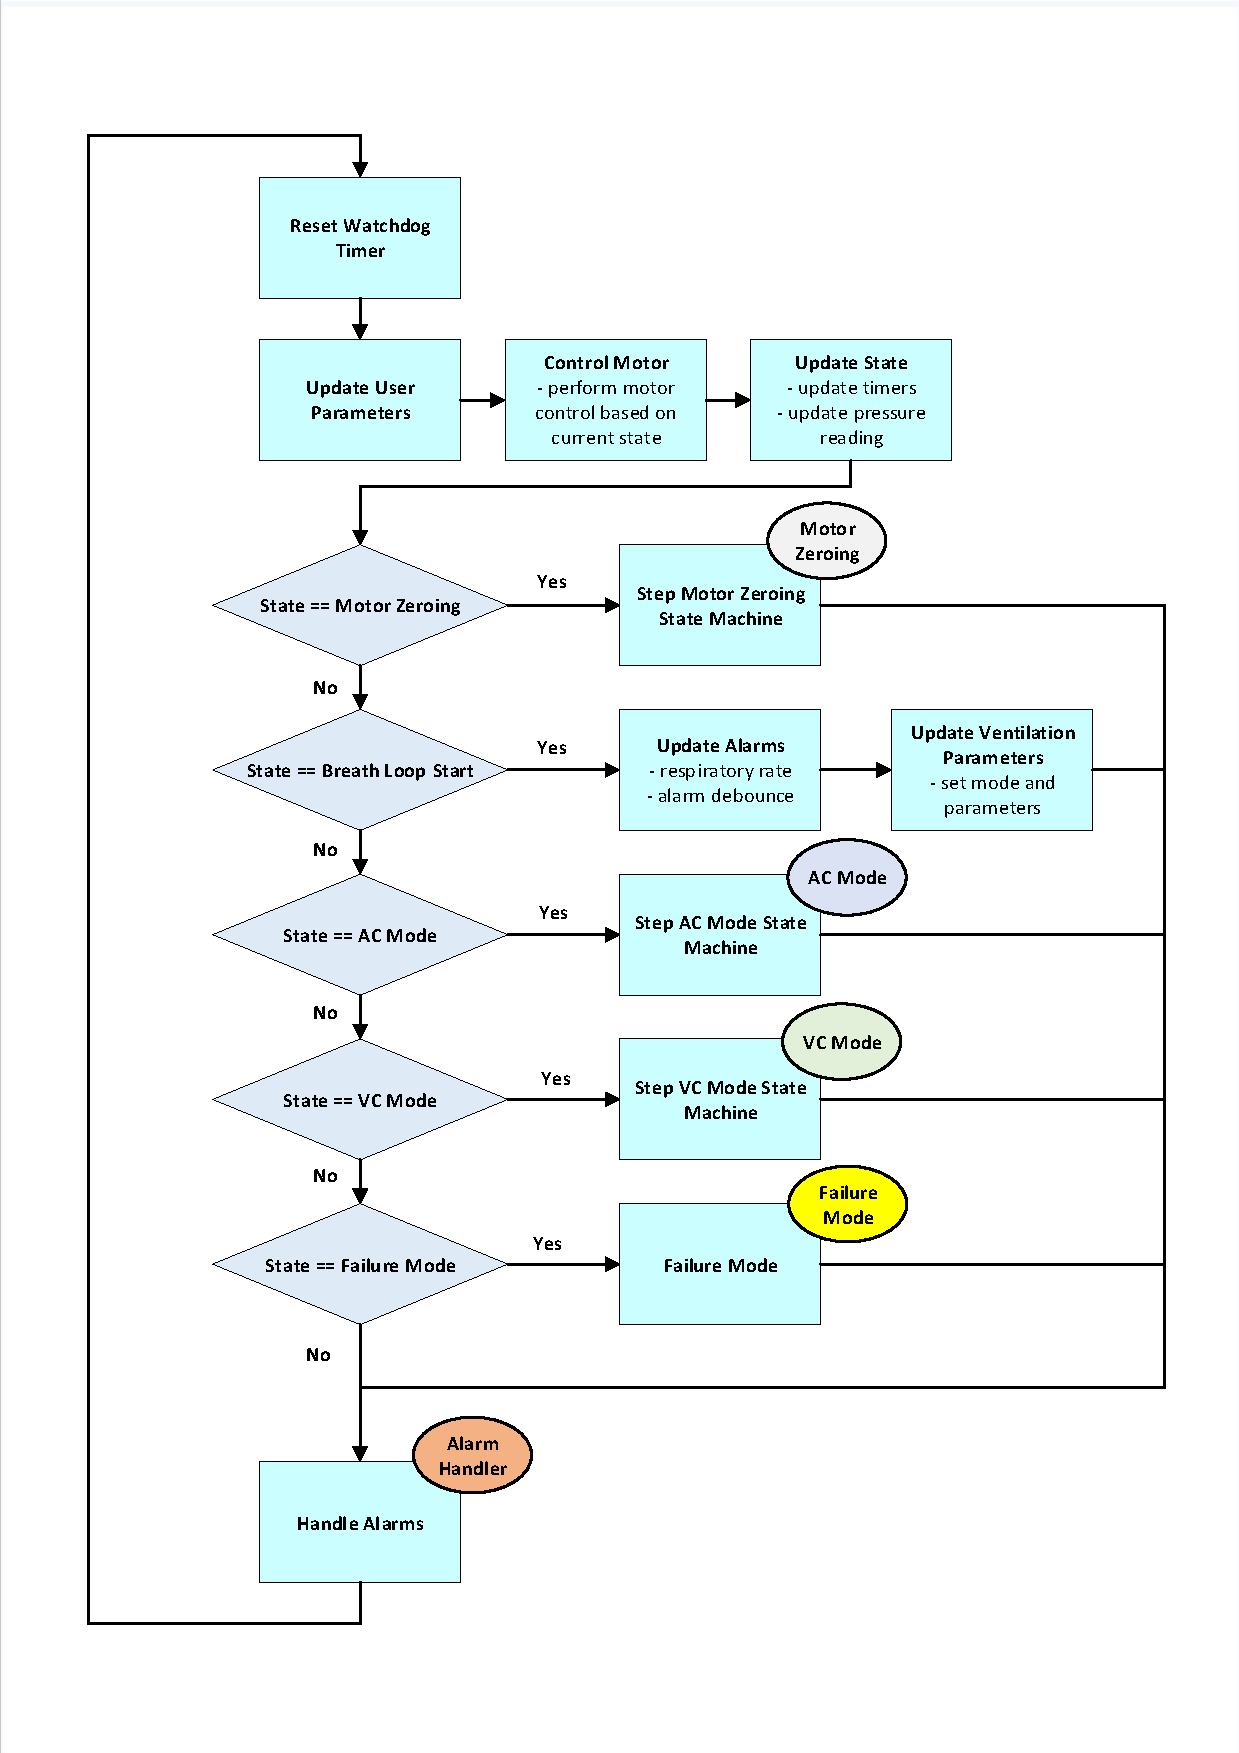
\includegraphics[scale= 0.82, trim=15 60 15 60, clip]{figures/main_loop.pdf}
	\caption{Main Program Loop}
	\label{fig:main_loop}
\end{figure}

\begin{sidewaysfigure}
	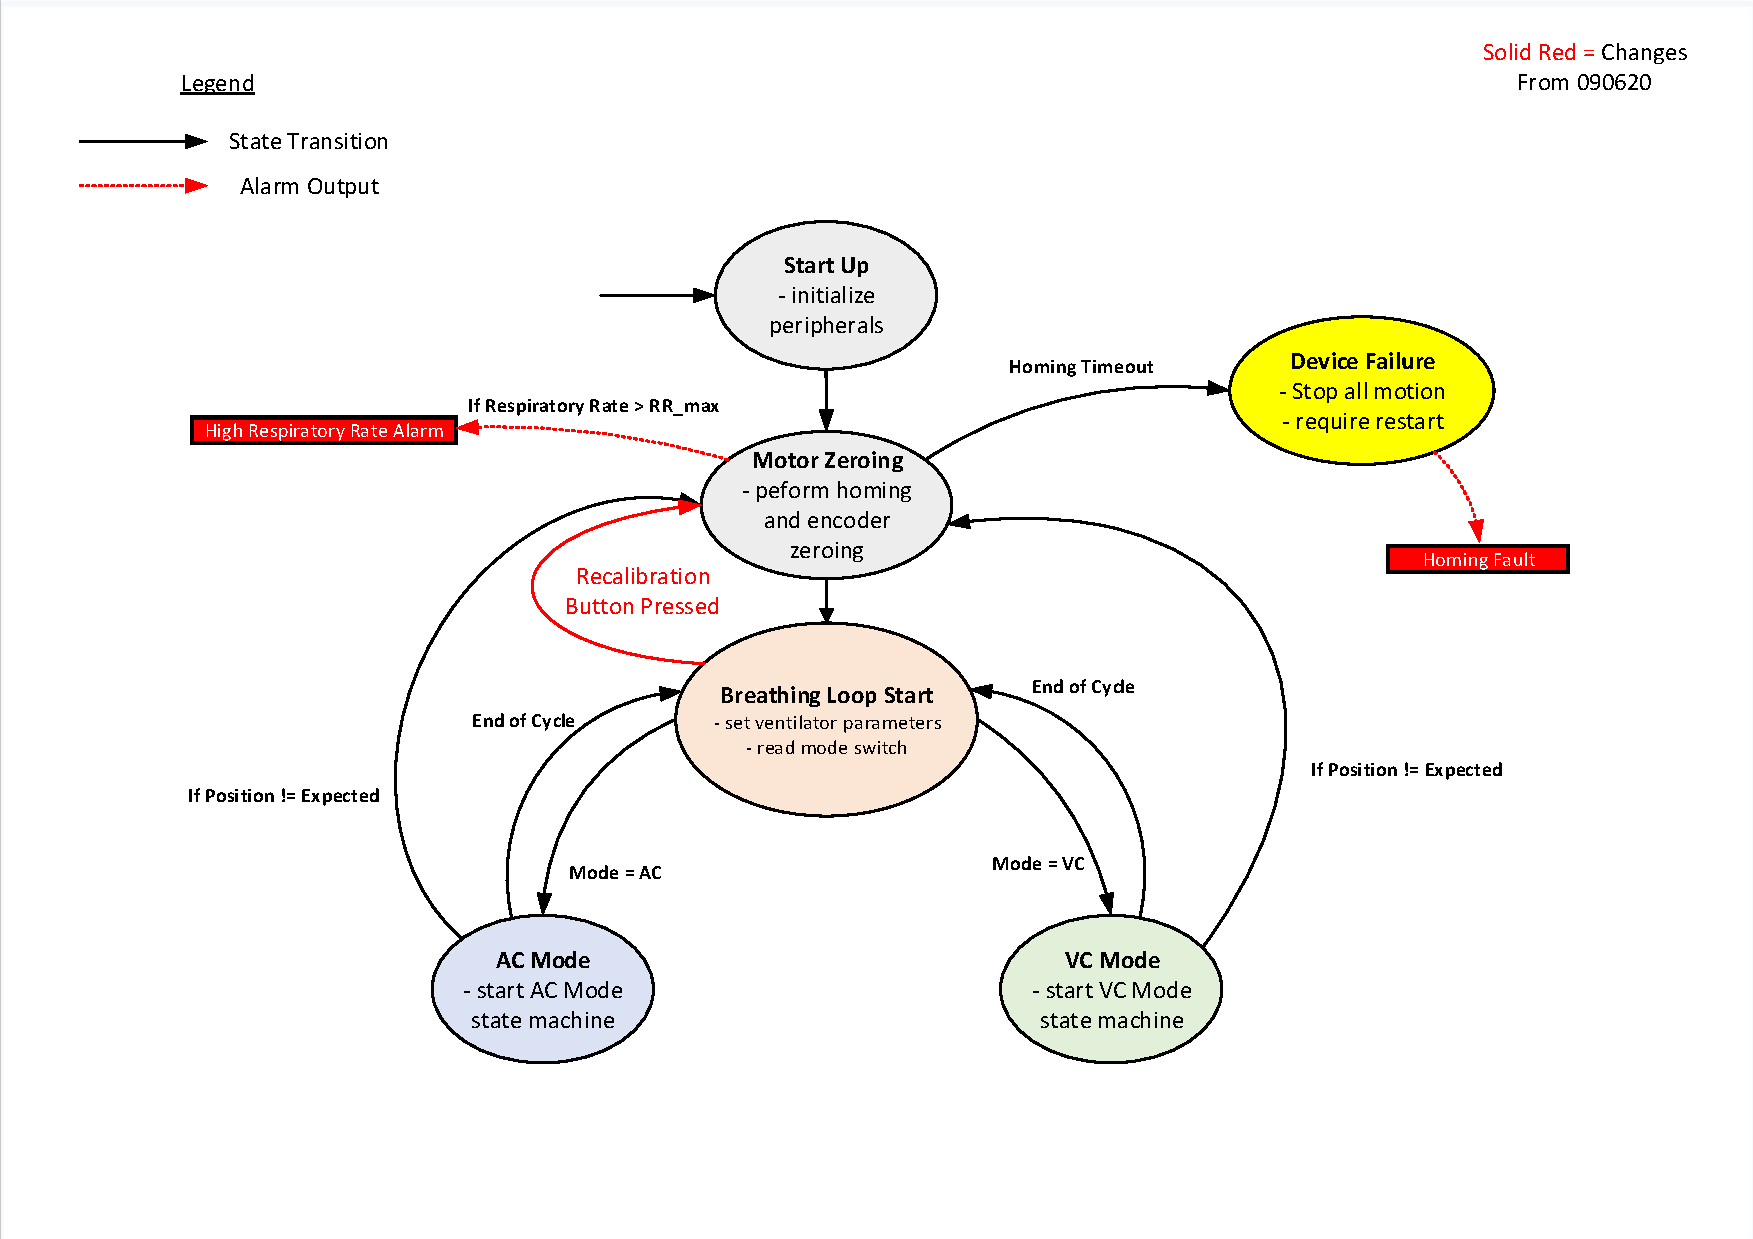
\includegraphics[scale=0.8, trim = 6 6 6 6, clip]{figures/main_state_flow.pdf}
	\caption{Overall Program State Flow Diagram}
	\label{fig:main_stfd}
\end{sidewaysfigure}

\begin{sidewaysfigure}
	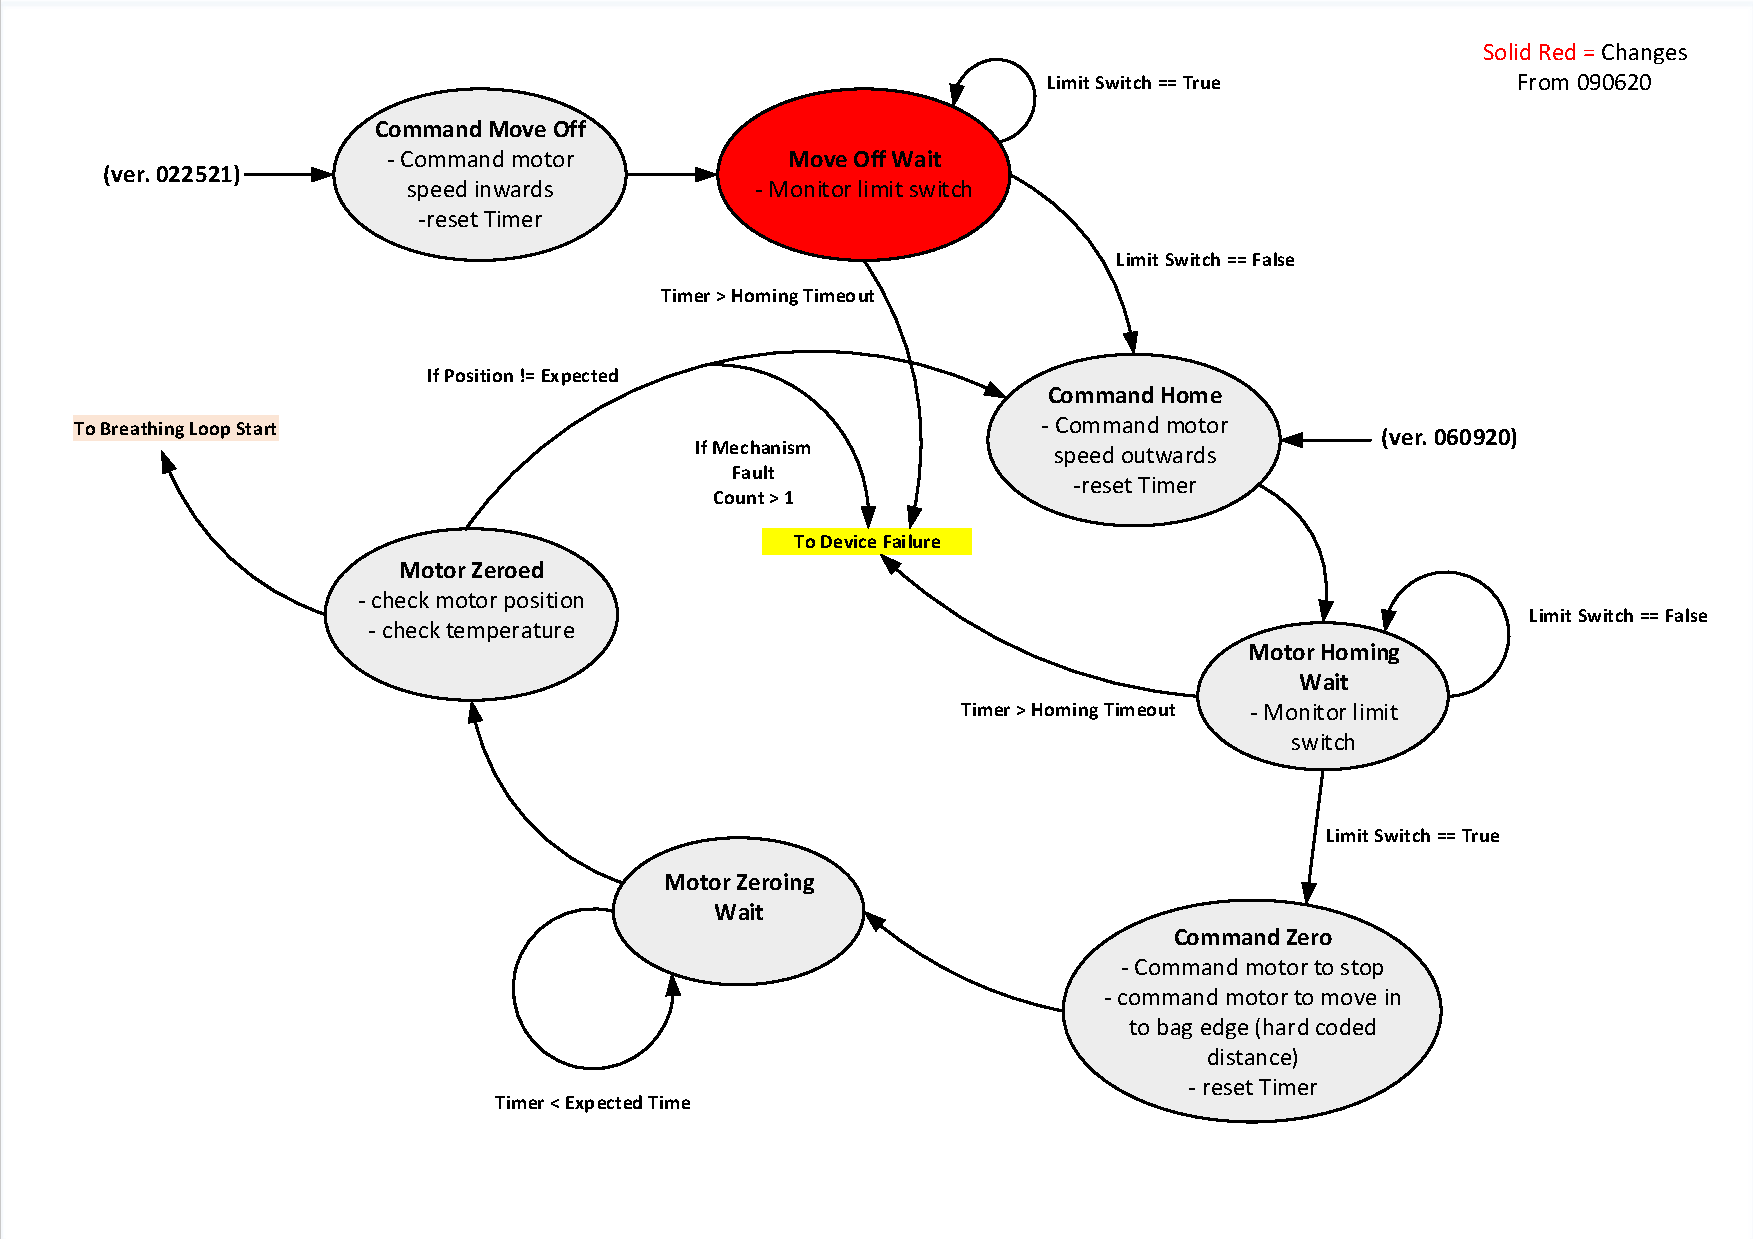
\includegraphics[scale=0.8, trim = 6 6 6 6, clip]{figures/motor_zeroing.pdf}
	\caption{Motor Zeroing State Flow Diagram}
	\label{fig:mz_stfd}
\end{sidewaysfigure}

\begin{sidewaysfigure}
	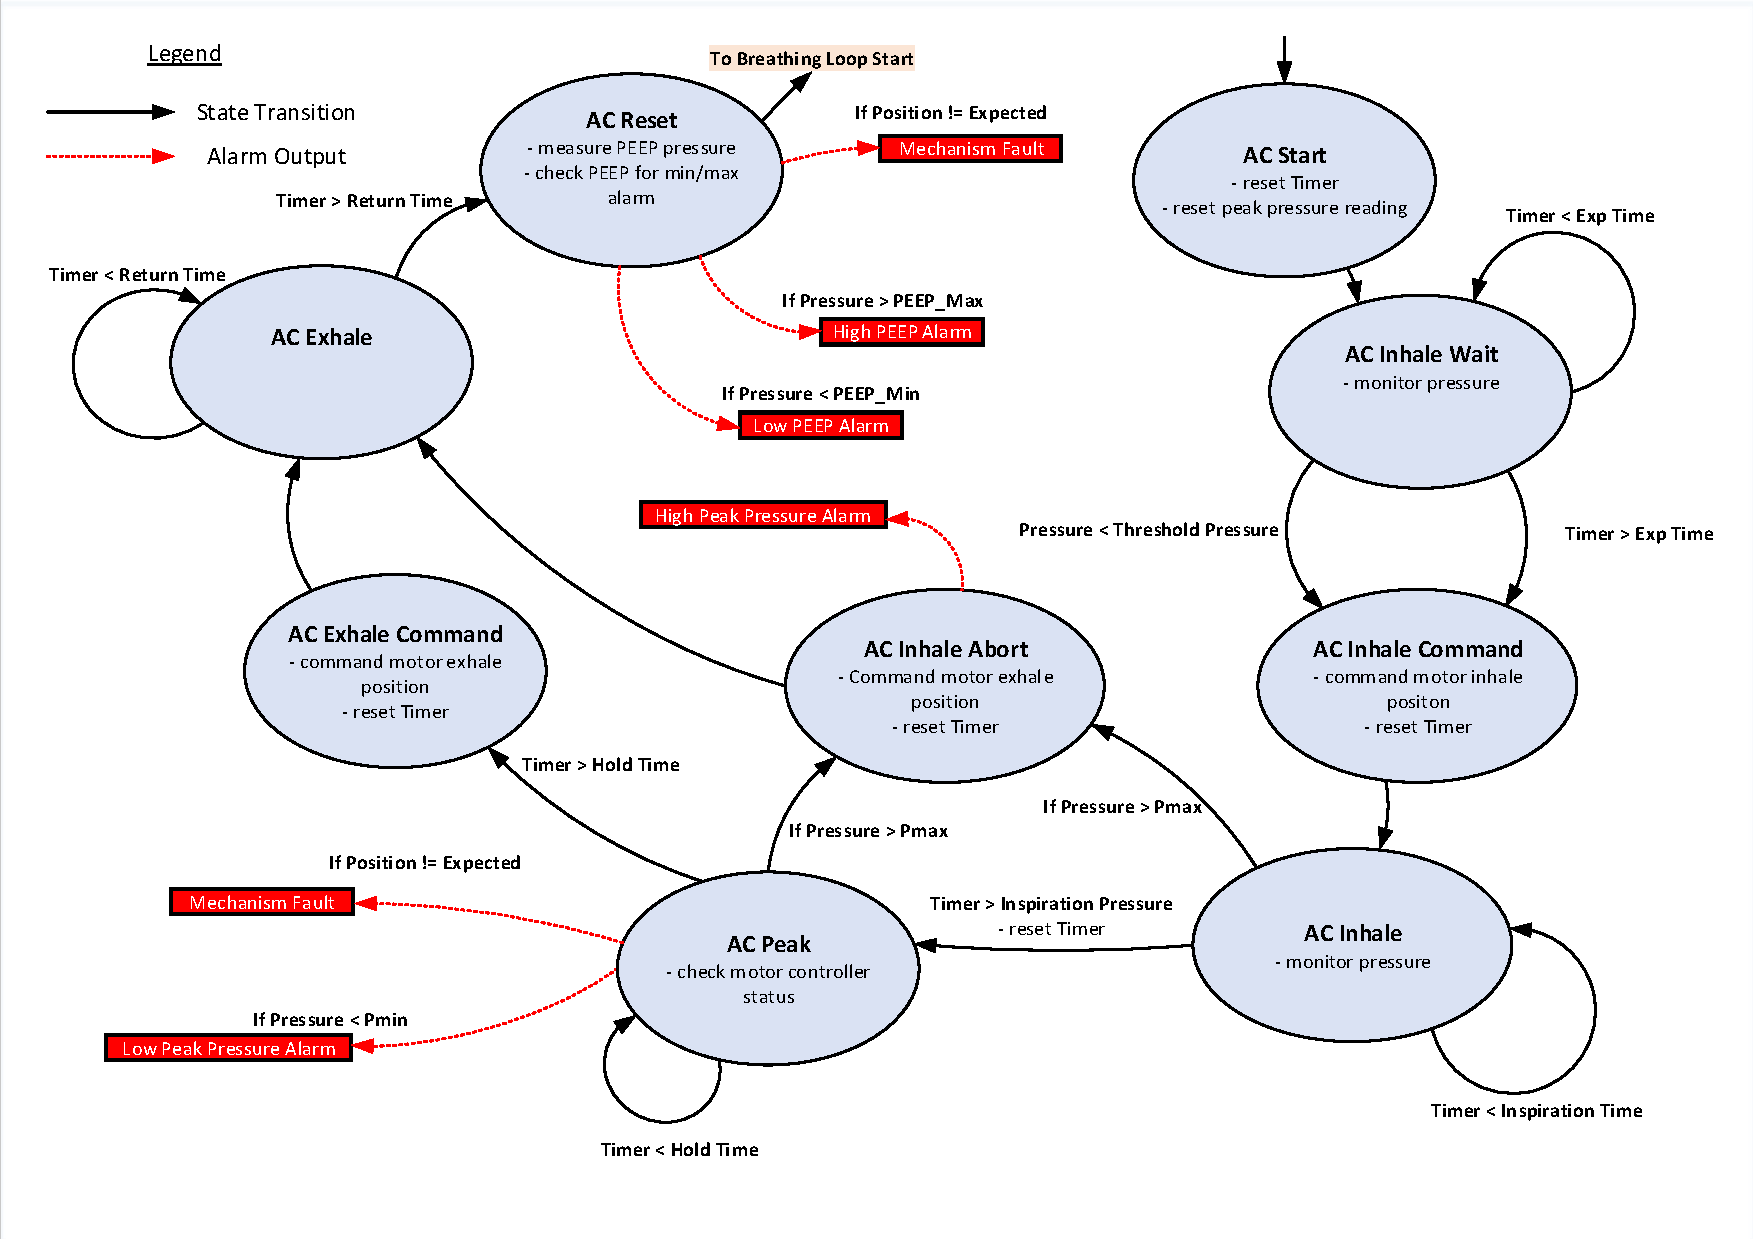
\includegraphics[scale=0.8, trim = 6 6 6 6, clip]{figures/ac_mode.pdf}
	\caption{Assist Control Mode State Flow Diagram}
	\label{fig:ac_stfd}
\end{sidewaysfigure}

\begin{sidewaysfigure}
	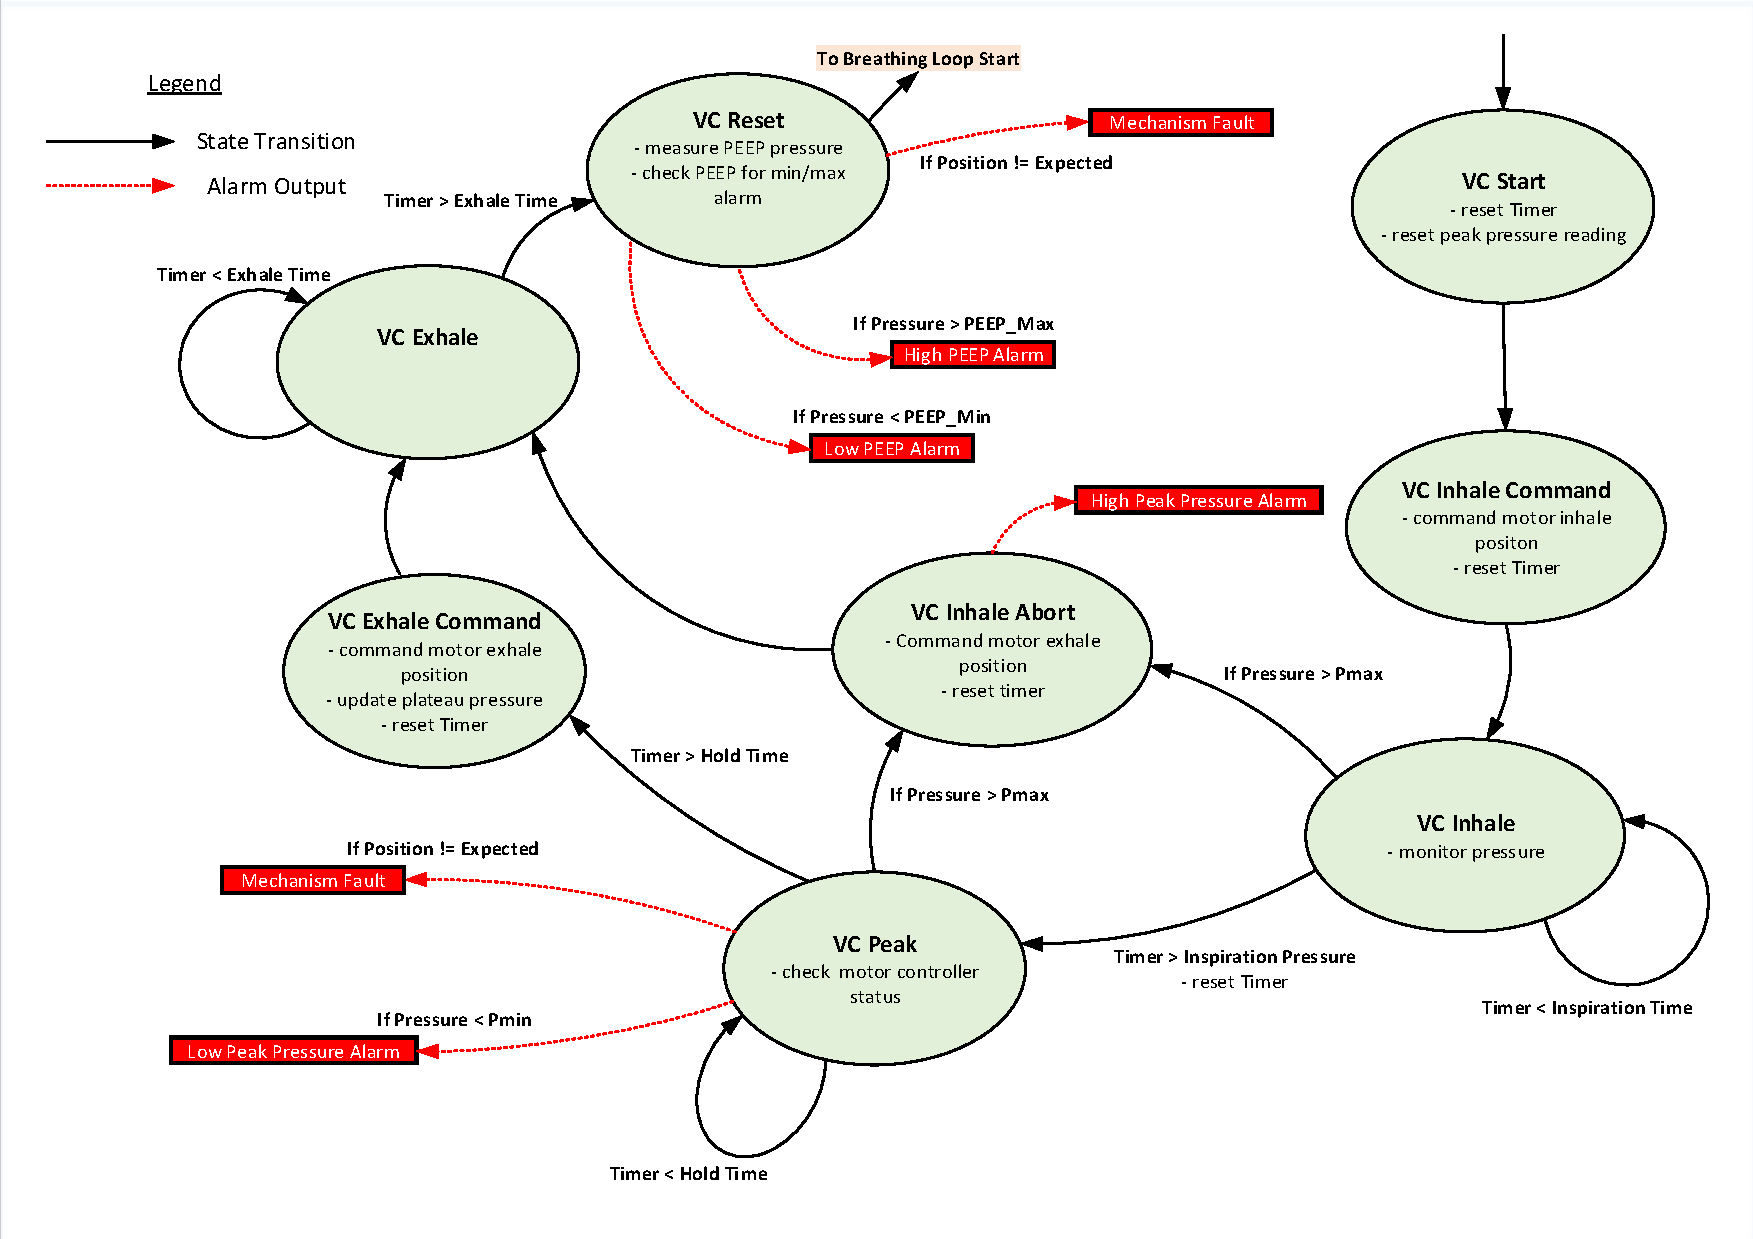
\includegraphics[scale=0.8, trim = 6 6 6 6, clip]{figures/vc_mode.pdf}
	\caption{Volume Control Mode State Flow Diagram}
	\label{fig:vc_stfd}
\end{sidewaysfigure}

\begin{figure}
	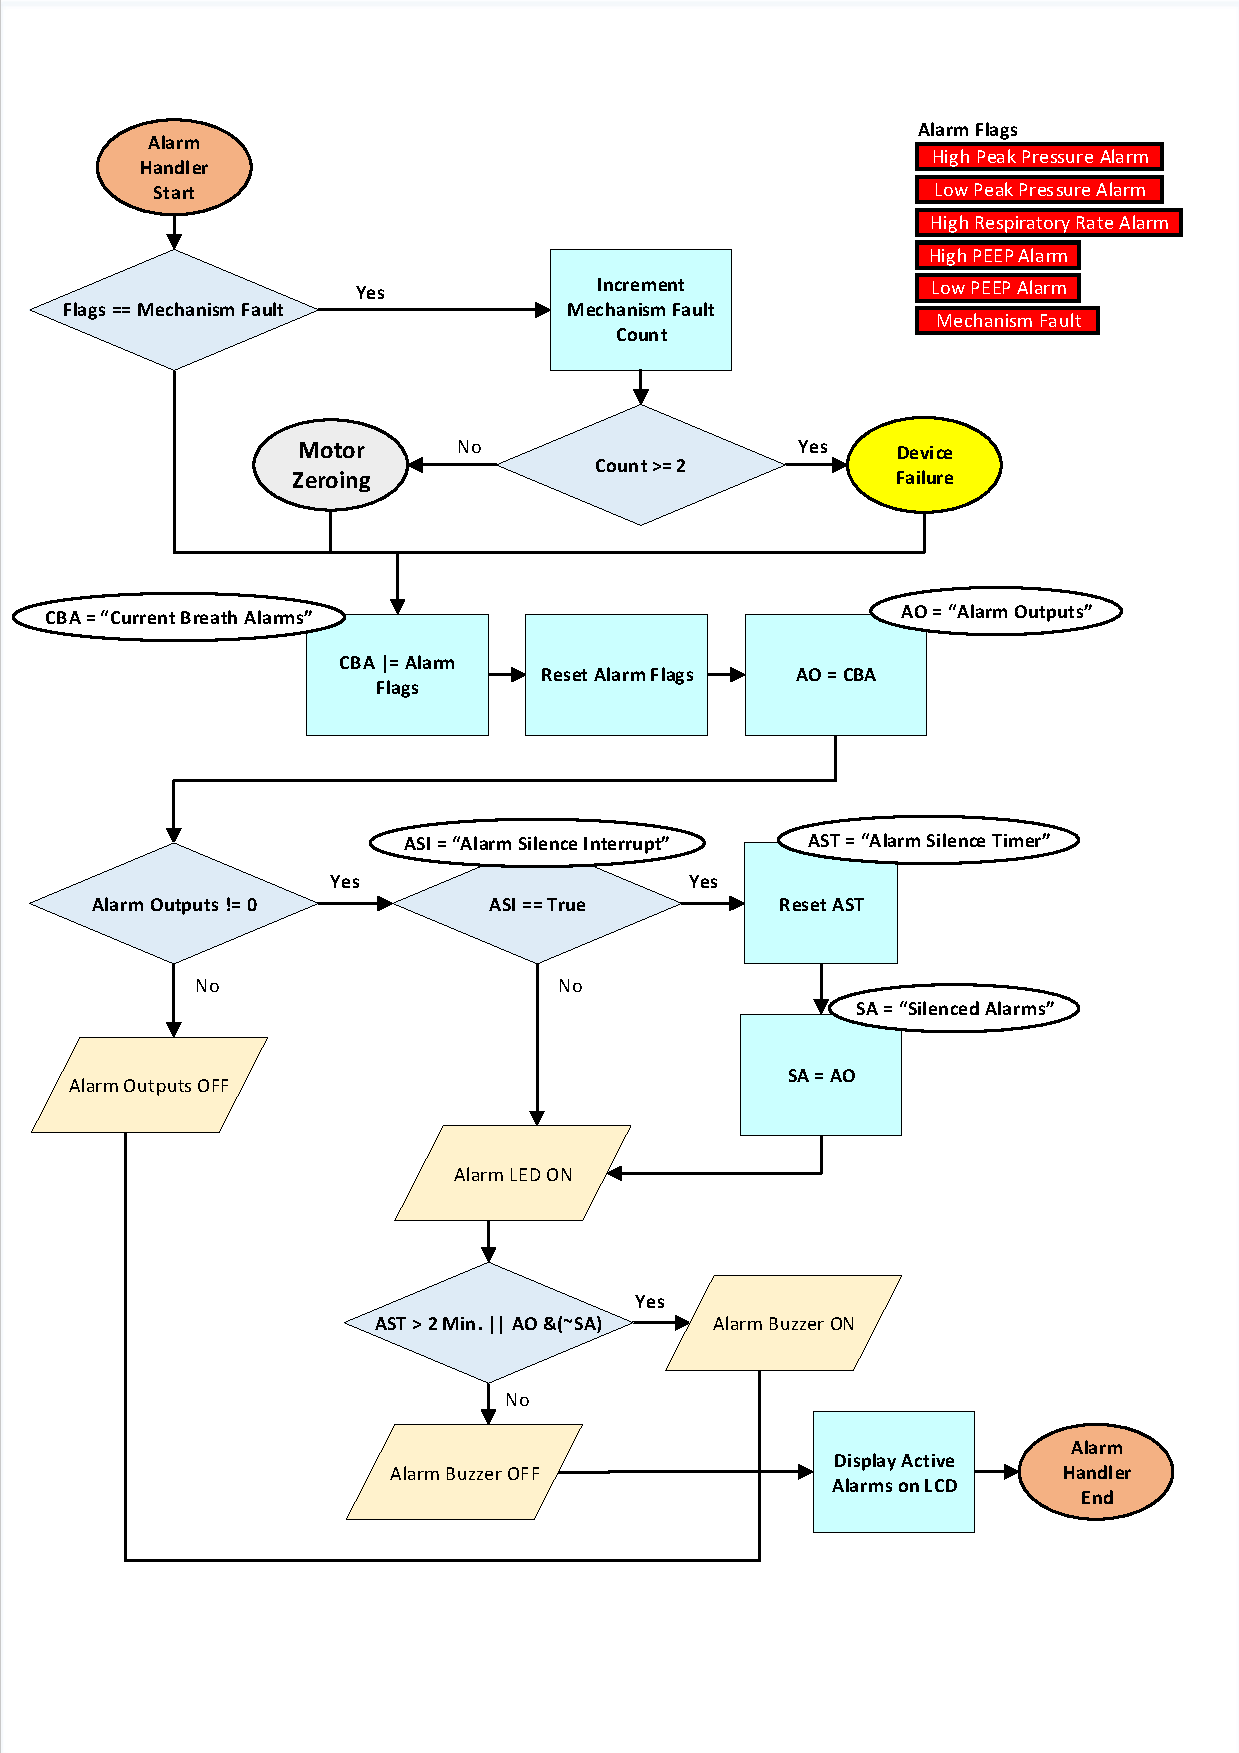
\includegraphics[scale= 0.82, trim=15 70 15 50, clip]{figures/alarm_handler.pdf}
	\caption{Alarm Handler}
	\label{fig:alarm_loop}
\end{figure}


\clearpage
\section{Risk Assessment}
The figures contained in this section outline the overall risk assessment of the ventilator system. Not all of the analysis in this section pertains to the software aspect of the ventilator.  For an examination of the software-specific risk mitigation implemented refer to Section \ref{sect:risk} of this document.
This appendix provides the following Figures:
\begin{itemize}
	\item Figure \ref{fig:risk_matrix} provides the risk matrix utilized in evaluation of the risk associated with the ventilator system.  The risk matrix employed is based on the ISO 14971 standard.
	\item Figures \ref{fig:unmit1} through \ref{fig:unmit3} outline the unmitigated risk associated with the ventilator.
	\item Figures \ref{fig:mit1} through \ref{fig:mit4} detail the risk mitigation steps that have been taken to minimize risk.
\end{itemize}

\begin{sidewaysfigure}
	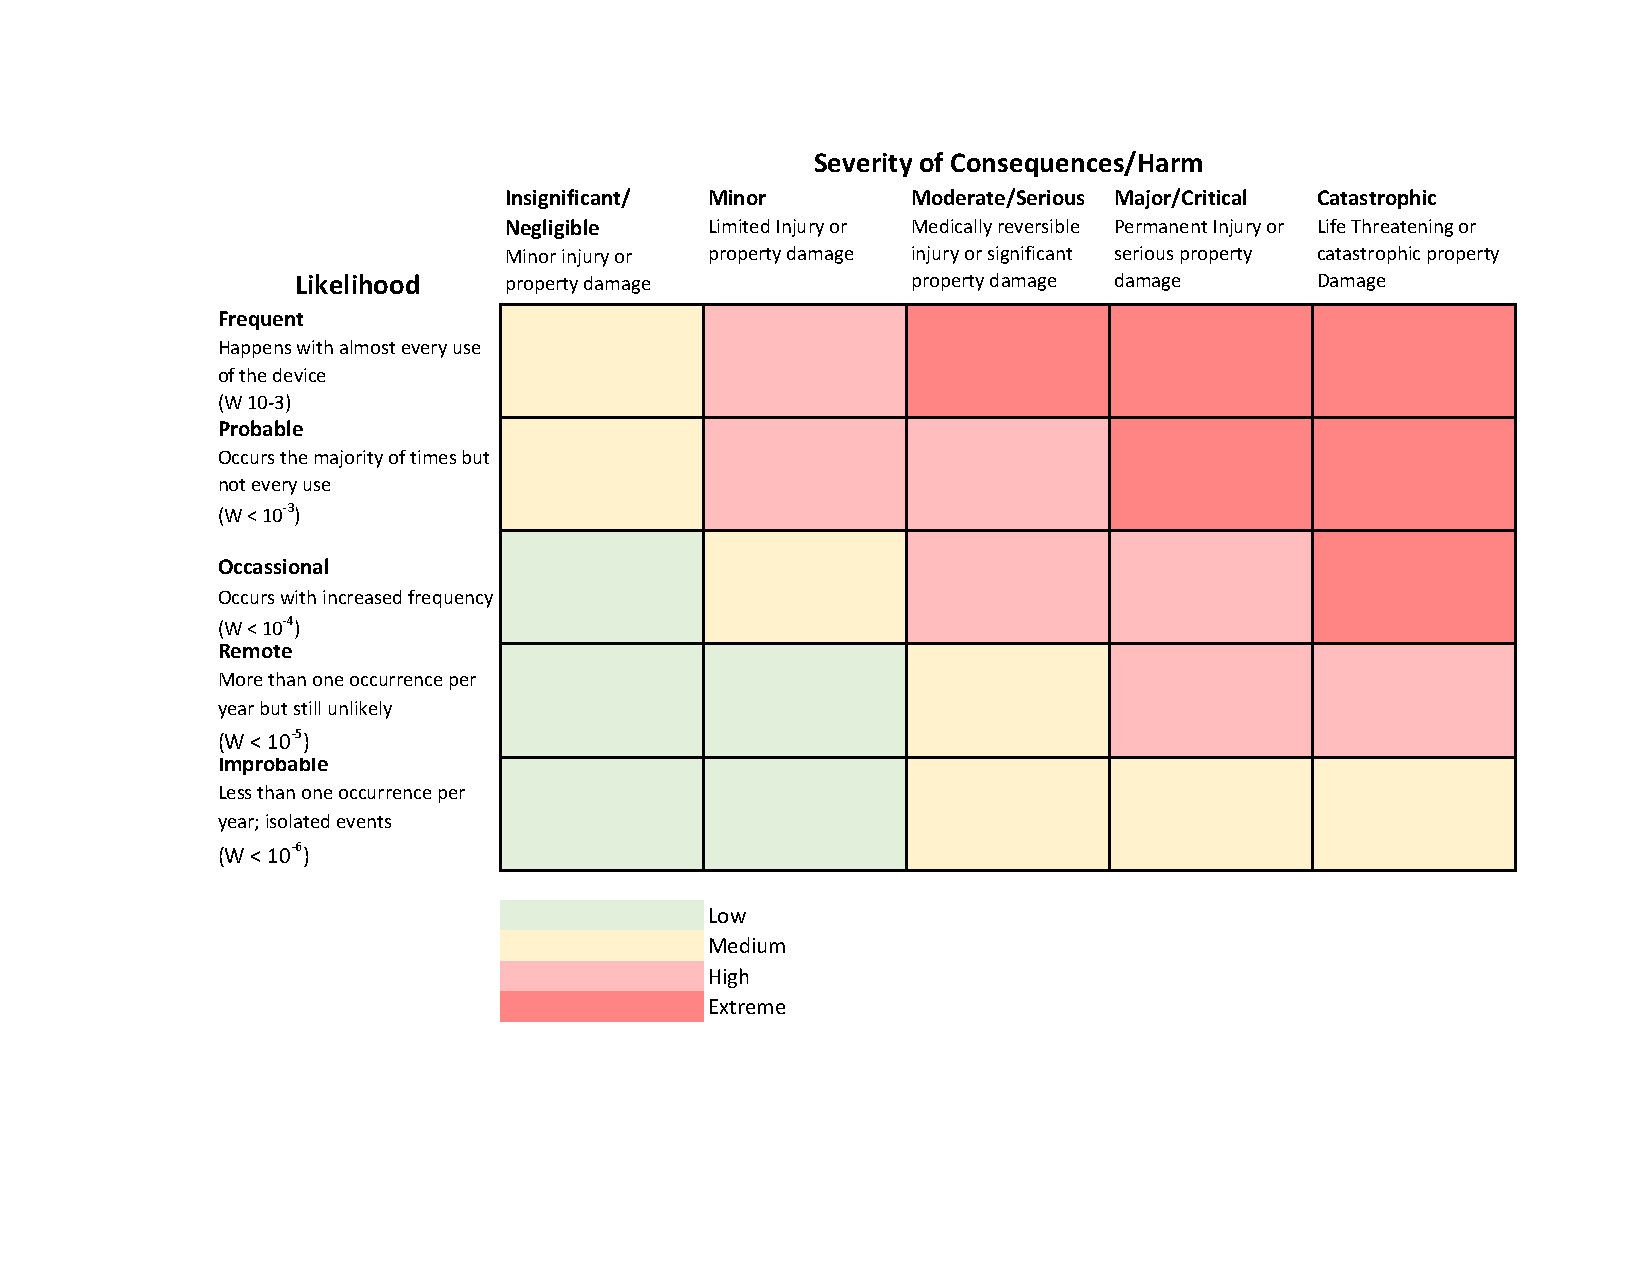
\includegraphics[scale= 0.9, trim=80 100 40 60, clip]{figures/risk_matrix.pdf}
	\caption{Risk Matrix based on ISO 14971 }
	\label{fig:risk_matrix}
\end{sidewaysfigure}

\begin{sidewaysfigure}
	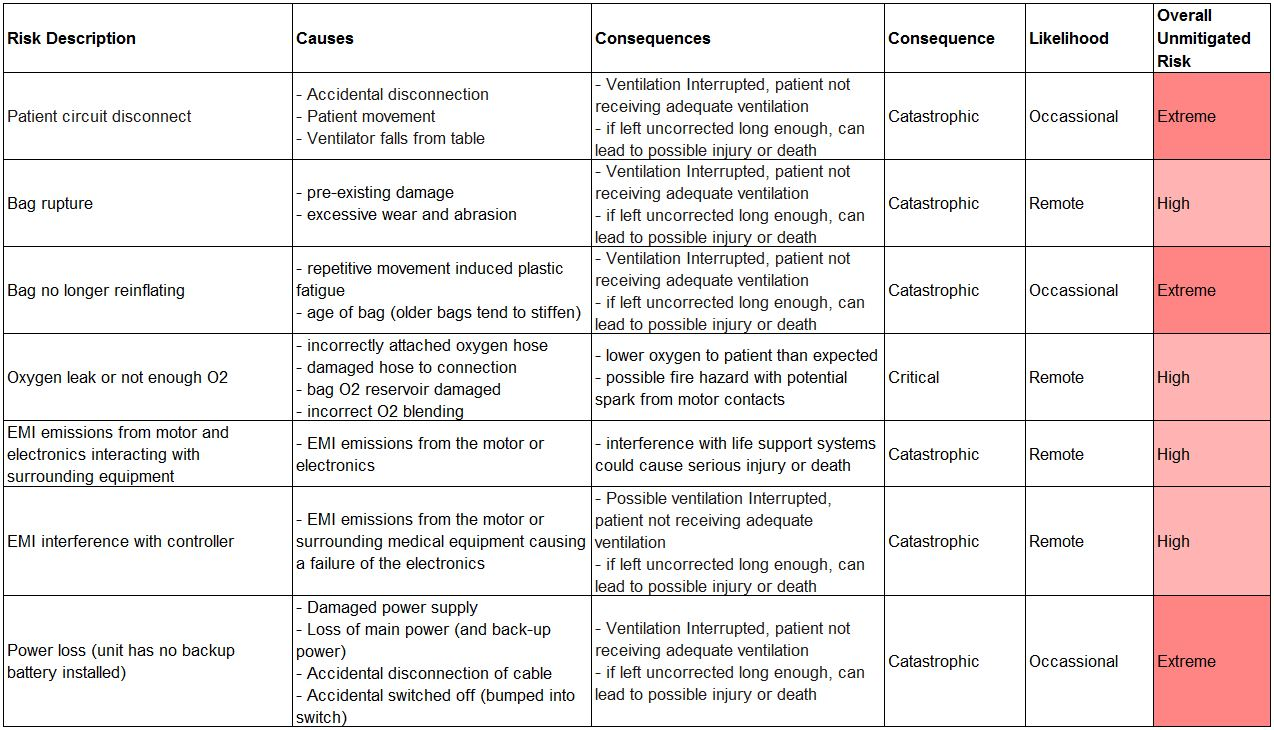
\includegraphics[scale= 0.6]{figures/unmit_1.jpg}
	\caption{Unmitigated Risk Analysis}
	\label{fig:unmit1}
\end{sidewaysfigure}

\begin{sidewaysfigure}
	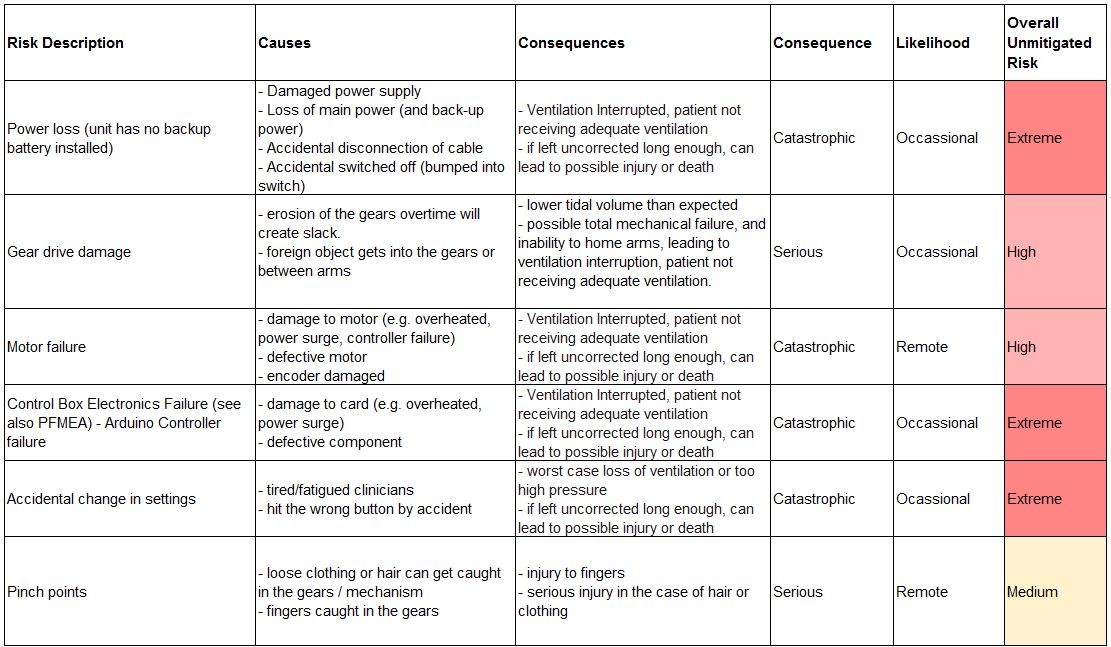
\includegraphics[scale= 0.65]{figures/unmit_2.jpg}
	\caption{Unmitigated Risk Analysis}
	\label{fig:unmit2}
\end{sidewaysfigure}

\begin{sidewaysfigure}
	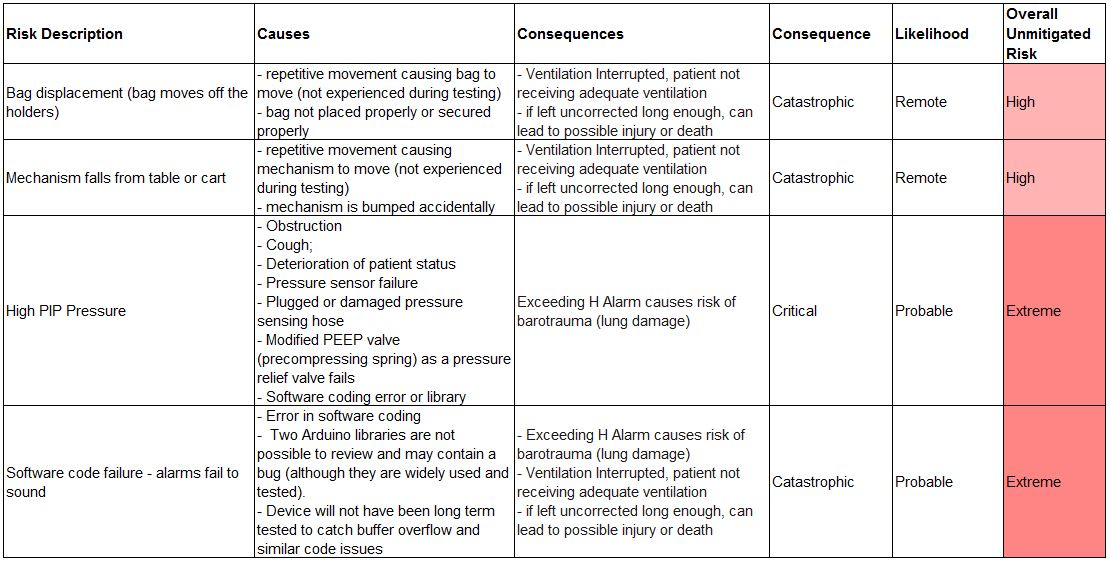
\includegraphics[scale= 0.7]{figures/unmit_3.jpg}
	\caption{Unmitigated Risk Analysis}
	\label{fig:unmit3}
\end{sidewaysfigure}



\begin{sidewaysfigure}
	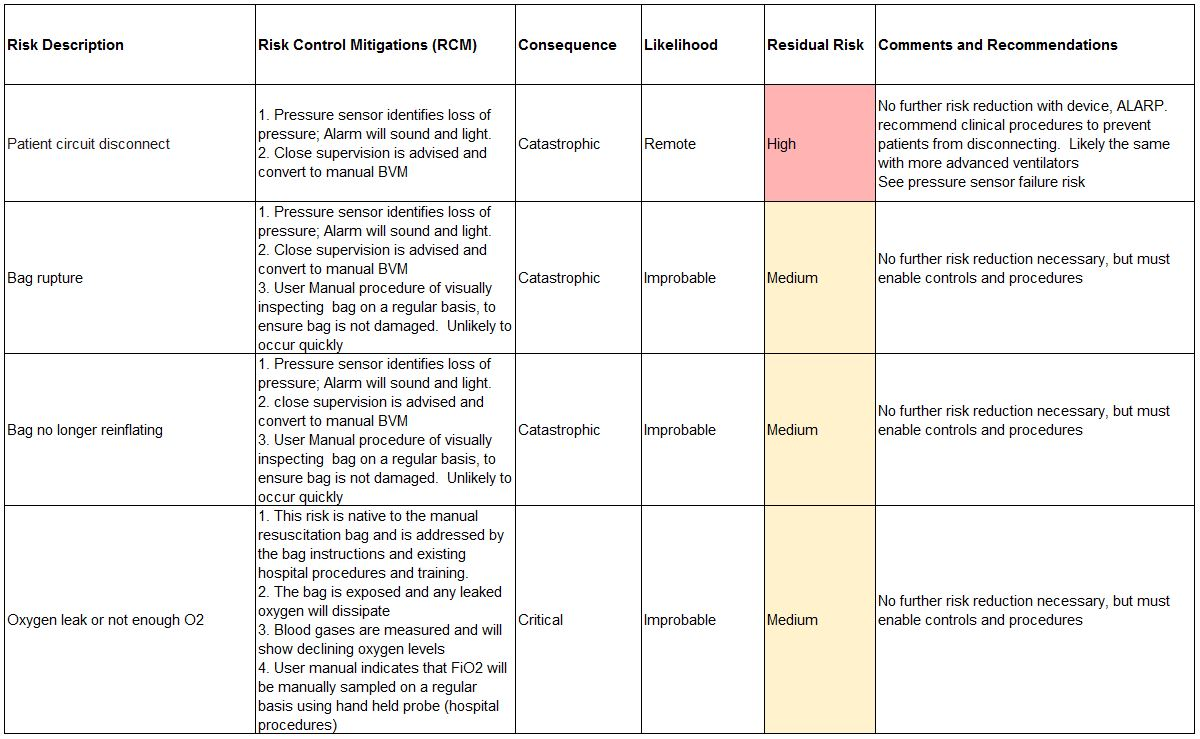
\includegraphics[scale= 0.66]{figures/mit1.jpg}
	\caption{Mitigated Risk Analysis}
	\label{fig:mit1}
\end{sidewaysfigure}

\begin{sidewaysfigure}
	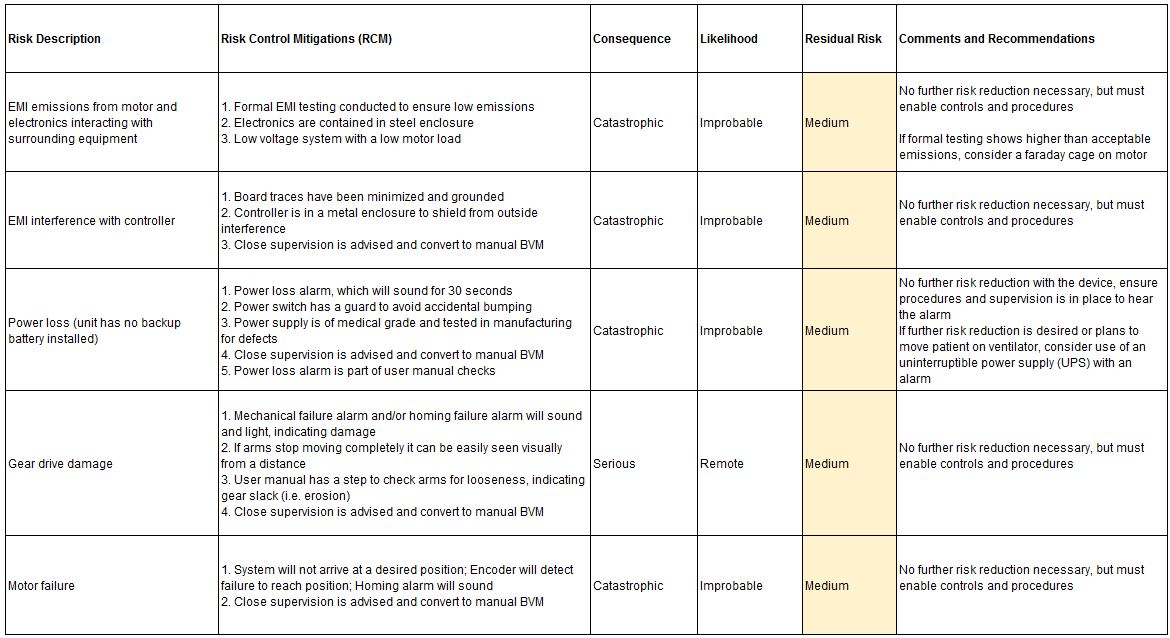
\includegraphics[scale= 0.7]{figures/mit2.jpg}
	\caption{Mitigated Risk Analysis}
	\label{fig:mit2}
\end{sidewaysfigure}

\begin{sidewaysfigure}
	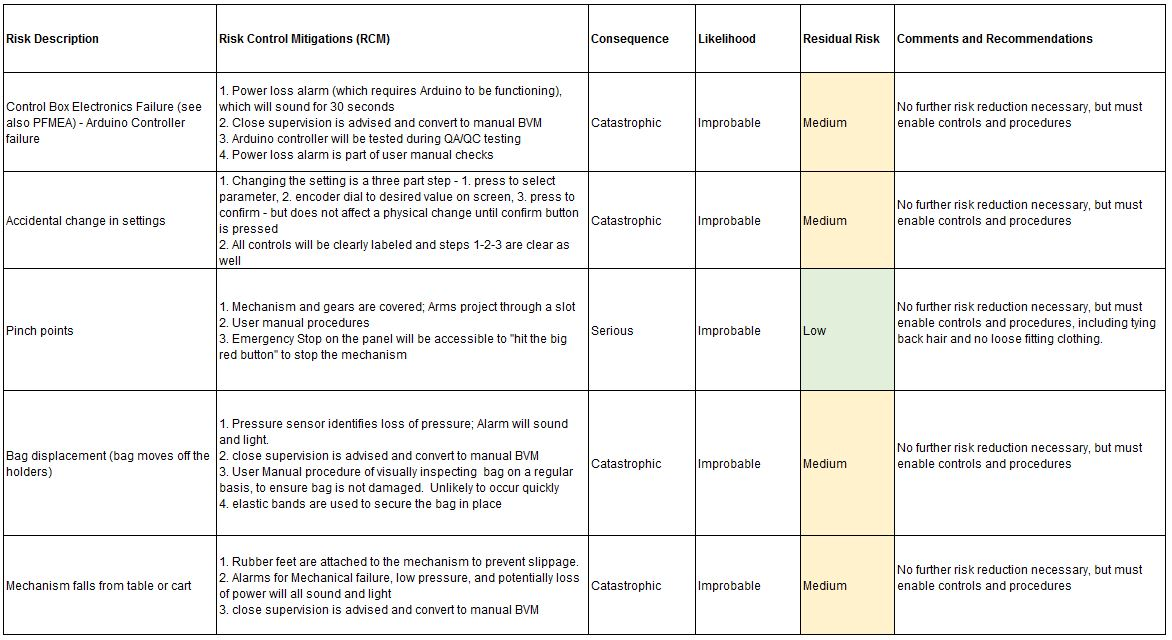
\includegraphics[scale= 0.7]{figures/mit3.jpg}
	\caption{Mitigated Risk Analysis}
	\label{fig:mit3}
\end{sidewaysfigure}

\begin{sidewaysfigure}
	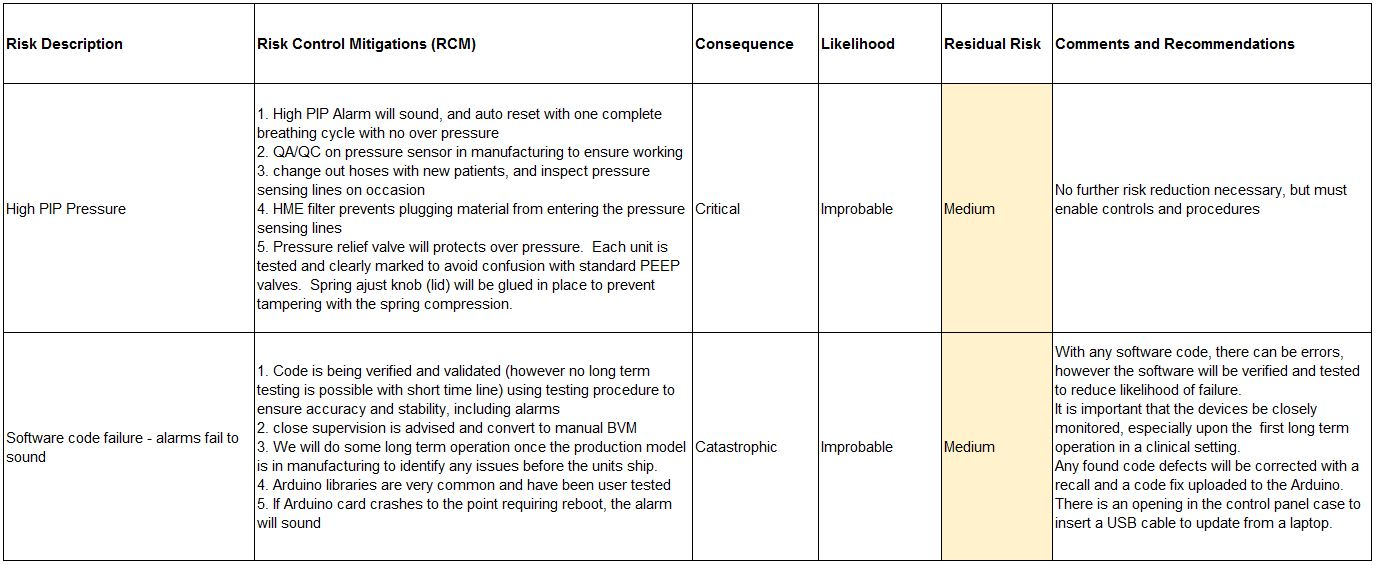
\includegraphics[scale= 0.6]{figures/mit4.jpg}
	\caption{Mitigated Risk Analysis}
	\label{fig:mit4}
\end{sidewaysfigure}


\clearpage
\section{Software Change Request Tracking}
\label{app:change}
The figures contained in this section are examples of the documentation that will used to track changes made to the Alberta E-Vent software.  These records will be maintained as part of the software repository and will provide traceability for all modifications that are made to the software.

\begin{sidewaysfigure}
	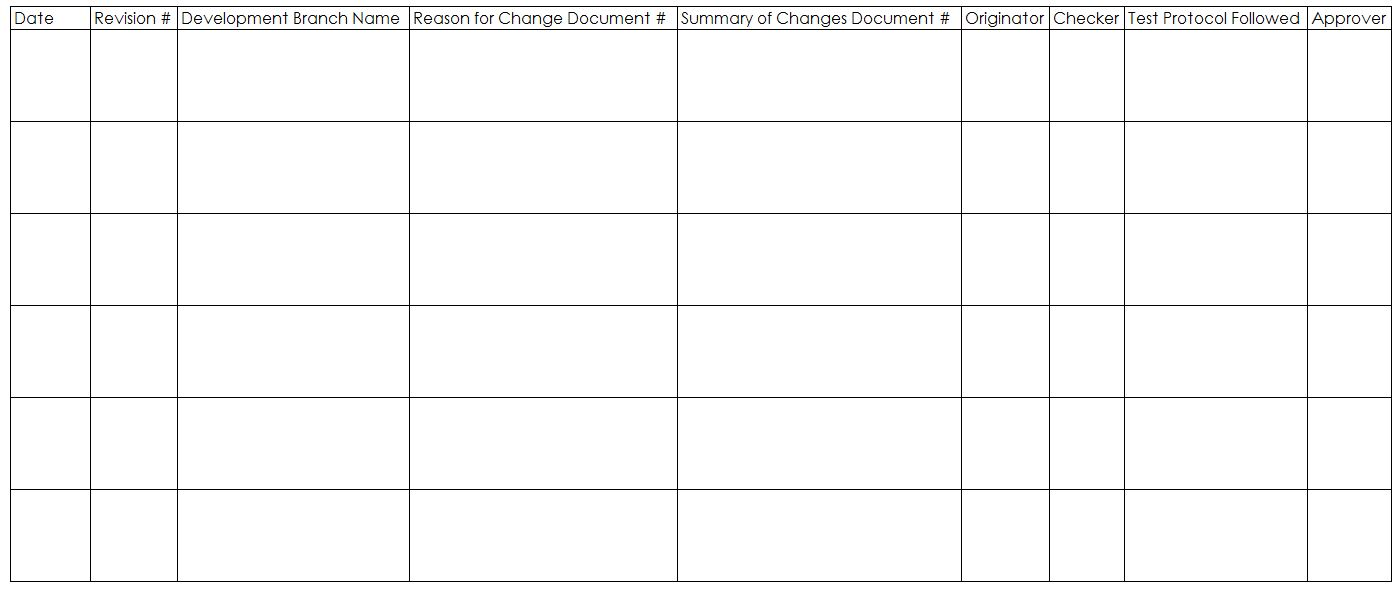
\includegraphics[scale= 0.6]{figures/change.jpg}
	\caption{Software Change Request Tracking}
	\label{fig:change_tracking}
\end{sidewaysfigure}

\end{appendices}
\end{document}
